%======================================================================
\chapter{Plasticity: yield, flow and generalized standard materials}\label{ch:pl}
%======================================================================
% Sources: slides c03 "Plasticity" (2025), exercise sheet "Elastoplastic
% filaments" (MEC643, 2025), notes "Optimization and variational structures
% in computational plasticity" (Ch. 1), "Global-local plasticity" (Sec. 1),
% "Exercises in computational inelasticity" (Parts 1 and 5),
% exercise "Stretching of an elastoplastic sheet" (MEC563, 2025),
% MEALOR II Ch. 2 (Kondo and Maitournam, 2023).
% Chapters 5 and 6 are referred to by number until they exist (then use \ref).

\framepart{Outline}
Metals loaded beyond a threshold keep a permanent deformation after unloading and dissipate energy. This chapter builds the classical theory of rate-independent plasticity in small strains. We follow the route of Simo and Hughes~\cite{SimoHughes1998}: the model is first written for a filament, where every ingredient can be computed by hand, and then for a three-dimensional body. The same model is then rewritten in the language of generalized standard materials of Halphen and Nguyen~\cite{HalphenNguyen1975}: a free energy and a convex dissipation potential. This rewriting shows that the flow rule is the optimality condition of a maximization, the principle of maximum plastic dissipation. Its convexity gives the main properties of the elastoplastic boundary-value problem: uniqueness of the stresses, a minimum principle for the rates, and bounds on the limit load. The integration of the model in time is the subject of Chapter~5.

\paragraph{By the end of this chapter you should be able to:}
\begin{itemize}
  \item describe the experimental facts behind plasticity (yield, hardening,
  unloading, Bauschinger effect) and the three ingredients of a model:
  elastic domain, flow rule and hardening rule;
  \item write the equations of an elastoplastic filament with isotropic and
  kinematic hardening, use the Kuhn--Tucker and consistency conditions, and
  compute the plastic multiplier and the tangent modulus;
  \item write the von Mises and Tresca criteria, the associative flow rule and
  the continuum elastoplastic tangent $\bbCep$ in three dimensions;
  \item identify the free energy, the state laws, the dissipation and the
  dissipation potential of a model, and translate between the notation of
  Simo and Hughes and that of generalized standard materials;
  \item state the principle of maximum plastic dissipation and derive from it
  the normality rule, the convexity of the elastic domain and the
  monotonicity of the flow rule;
  \item formulate the elastoplastic boundary-value problem, prove the
  uniqueness of the stresses, and bound the limit load from below and above.
\end{itemize}

\paragraph{Plan of the chapter.} Section~\ref{sec:pl-intro} recalls the experimental facts. Section~\ref{sec:pl-1d} treats the elastoplastic and the viscoplastic filament. Section~\ref{sec:pl-3d} extends the model to three dimensions, with the von Mises and Tresca criteria and the continuum tangent. Section~\ref{sec:pl-gsm} introduces thermodynamics and generalized standard materials, and Section~\ref{sec:pl-maxdiss} the principle of maximum plastic dissipation. Section~\ref{sec:pl-bvp} states the boundary-value problem and its main properties. A summary, exercises with solutions (page~\pageref{sec:pl-exo}) and the references close the chapter. Classical references are~\cite{SimoHughes1998,Lubliner1990,LemaitreChaboche1990,Salencon2002,Maitournam2012} for the mechanics, \cite{KondoMaitournam2023} for the thermodynamic formulation, and~\cite{HanReddy2013,Temam1983,Nguyen2000} for the mathematics.

\begin{gbox}{Guiding questions}
\begin{enumerate}[itemsep=1pt]
  \item Which experiments define plasticity, and which quantities must a
  model carry to reproduce them? (Section~\ref{sec:pl-intro})
  \item How does one decide, at a given instant, whether the material loads
  plastically or unloads elastically, and how fast the plastic strain grows?
  (Sections~\ref{sec:pl-1d}--\ref{sec:pl-3d})
  \item Which part of the work is stored and which part is dissipated, and
  why is the elastic domain convex? (Sections~\ref{sec:pl-gsm}--\ref{sec:pl-maxdiss})
  \item Is the response of a structure unique, and up to which load can it
  carry? (Section~\ref{sec:pl-bvp})
\end{enumerate}
The tools are those of Chapters~\ref{ch:var} and~\ref{ch:elliptic}: the
equations of elasticity, the virtual work principle, the Legendre--Fenchel
transform (Section~\ref{sec:var-dual}) and the Karush--Kuhn--Tucker conditions
(Section~\ref{sec:var-lagrange}).
\end{gbox}

%======================================================================
\section{Plasticity in experiments}\label{sec:pl-intro}
\index{plasticity!experimental facts}\index{yield stress}\index{hardening}\index{Bauschinger effect}%
Plasticity is visible in two kinds of applications. In metal forming
(stamping, deep drawing, rolling, forging) the goal is a \emph{permanent
deformation}: the part must keep its new shape after the tools are removed. In
crash or impact protection the goal is \emph{energy dissipation}: a structure
absorbs the kinetic energy of an impact by deforming plastically. Both
features appear in the simplest experiment, the tensile test
(Figure~\ref{fig:pl-tension}).

\begin{figure}[h]
\centering
\begin{tikzpicture}[scale=1.0,>=Latex]
  \draw[->] (-0.3,0) -- (7.4,0) node[right] {$\varepsilon$};
  \draw[->] (0,-2.6) -- (0,3.3) node[above] {$\sigma$};
  % monotone curve with hardening
  \draw[very thick,cu] (0,0) -- (0.8,1.6);
  \draw[very thick,cu] (0.8,1.6) .. controls (1.5,2.15) and (2.6,2.45) .. (3.6,2.6);
  % unloading-reloading
  \draw[very thick,cphi] (3.6,2.6) -- (2.3,0) node[below right,black] {$\varepsilon^p$};
  \draw[thick,cphi,dashed] (2.3,0) -- (1.6,-1.4);
  \draw[very thick,orange!80!black] (1.6,-1.4) .. controls (1.3,-1.75) and (0.9,-1.95) .. (0.3,-2.1);
  \draw[very thick,cu,dashed] (3.6,2.6) .. controls (4.6,2.75) and (5.8,2.9) .. (7.0,3.0);
  % labels
  \draw[dashed,gray] (0,1.6) node[left,black] {$\sY$} -- (0.8,1.6);
  \draw[dashed,gray] (0,2.6) node[left,black] {$\sigma_1$} -- (3.6,2.6);
  \draw[dashed,gray] (0,-1.4) node[left,black] {$\sigma_2$} -- (1.6,-1.4);
  \node[font=\small,align=left,anchor=west] at (3.6,1.2) {unloading and reloading\\ are elastic, slope $E$};
  \draw[->,gray] (3.55,1.2) -- (3.0,1.2);
  \node[font=\small,align=left] at (4.3,-1.6) {reverse yielding at\\ $|\sigma_2|<\sigma_1$ (Bauschinger)};
  \node[font=\small] at (1.45,2.75) {hardening};
  \node[font=\small,cu] at (0.55,0.45) {$E$};
\end{tikzpicture}
\caption{Tensile test on a metal (schematic). Beyond the yield stress $\sY$
the response is nonlinear and the stress keeps increasing (hardening).
Unloading is elastic and leaves a permanent strain $\varepsilon^p$. Reloading
follows the unloading line up to the previous maximum stress $\sigma_1$. In
compression, yielding starts again at a stress $|\sigma_2|$ smaller than
$\sigma_1$: this is the Bauschinger effect.}
\label{fig:pl-tension}
\end{figure}

The tensile test shows five facts.
\begin{itemize}
  \item \emph{Elastic range.} Below the \emph{yield stress} $\sY$ the response
  is linear and reversible, with Young's modulus $E$.
  \item \emph{Hardening.} Beyond $\sY$ the stress needed to deform further
  increases with the deformation (work hardening). Without hardening the
  material is \emph{perfectly plastic}.
  \item \emph{Elastic unloading.} Unloading follows a straight line of slope
  $E$ and leaves a permanent \emph{plastic strain} $\varepsilon^p$. Reloading
  is elastic up to the highest stress reached before: the elastic range has
  grown.
  \item \emph{Bauschinger effect.} After a tensile plastic strain, yielding in
  compression starts at a stress smaller in magnitude than the stress reached
  in tension. The elastic range has moved.
  \item \emph{Rate independence.} At room temperature and for moderate strain
  rates the curve hardly depends on the loading rate. Time plays the role of a
  parameter that orders the events. At high temperature the response depends
  on the rate (viscoplasticity, Section~\ref{ssec:pl-vp1d}).
\end{itemize}

Multiaxial tests, such as tension--torsion of thin tubes or biaxial
tension of cruciform specimens, measure the stresses at which yielding starts
along different loading directions. The set of these stresses is the boundary
of the \emph{elastic domain} in stress space, the \emph{yield surface}. For
most metals it is well described by the von Mises or the Tresca criterion
(Section~\ref{ssec:pl-criteria}). After plastic loading the yield surface
expands (\emph{isotropic hardening}) and translates in the direction of the
loading (\emph{kinematic hardening}), and the plastic strain rate is normal to
it (\emph{normality}) \cite{Lubliner1990,Salencon2002}.
\draftnote{Experimental figures of the slides (tension--torsion yield loci of P.~Suquet's course, after H.~D.~Bui) are not reproduced; ask for permission or redraw from data.}

\begin{gbox}{Ingredients of a plasticity model}
\index{plasticity!ingredients of a model}%
\begin{enumerate}[itemsep=1pt]
  \item a \emph{decomposition} of the strain into an elastic and a plastic
  part, with an elastic law for the stress;
  \item an \emph{elastic domain}, defined by a yield function $f\le0$, inside
  which the response is elastic;
  \item a \emph{flow rule}, which gives the direction of the plastic strain
  rate, and \emph{loading/unloading conditions}, which decide whether it
  vanishes;
  \item a \emph{hardening rule}, which describes how the elastic domain changes
  with plastic deformation.
\end{enumerate}
\end{gbox}

%======================================================================
\section{The elastoplastic filament}\label{sec:pl-1d}
\index{filament}\index{plasticity!one-dimensional}%
A \emph{filament} is a thin homogeneous bar in tension--compression, for which
the transverse components of displacement, strain and stress can be
neglected. Its state is described by the axial displacement $u(x,t)$, the
strain $\displaystyle \varepsilon=\frac{\partial u}{\partial x}$, the stress
$\sigma$ and the plastic strain $\varepsilon^p$. Other internal variables are
added when hardening is modelled. All the structure of the three-dimensional
theory is already present in this setting~\cite[Ch.~1]{SimoHughes1998}.

\subsection{Perfect plasticity: the frictional device}\label{ssec:pl-1d-perfect}
\index{plasticity!perfect}\index{frictional device}%
The rheological model is a spring of stiffness $E$ in series with a Coulomb
friction element of threshold $\sY$ (Figure~\ref{fig:pl-rheo}). The friction
element does not move while $|\sigma|<\sY$, and slides in the direction of
the stress when $|\sigma|=\sY$. The total strain is the sum of the strain of
the spring and the slip of the friction element:
\begin{equation}\label{eq:pl-split1d}
  \varepsilon=\varepsilon^e+\varepsilon^p,\qquad \sigma=E\,\varepsilon^e=E(\varepsilon-\varepsilon^p).
\end{equation}

\begin{figure}[h]
\centering
\begin{tikzpicture}[scale=1.0,>=Latex]
  % wall
  \fill[pattern=north east lines] (-0.25,-0.6) rectangle (0,0.6);
  \draw[thick] (0,-0.6) -- (0,0.6);
  % spring E
  \draw[spring] (0,0) -- (2.0,0);
  \node[above] at (1.0,0.25) {$E$};
  % friction element
  \draw[thick] (2.0,0) -- (2.4,0);
  \draw[thick,fill=gray!20] (2.4,-0.35) rectangle (3.4,0.35);
  \draw[thick] (2.4,-0.5) -- (4.0,-0.5);
  \fill[pattern=north east lines] (2.4,-0.68) rectangle (4.0,-0.5);
  \node at (2.9,0) {$\sY$};
  \draw[thick] (3.4,0) -- (4.2,0);
  \draw[->,very thick] (4.2,0) -- (5.0,0) node[right] {$\sigma$};
  \draw[|<->|] (0,-1.1) -- (2.0,-1.1) node[midway,below] {$\varepsilon^e$};
  \draw[|<->|] (2.0,-1.1) -- (4.2,-1.1) node[midway,below] {$\varepsilon^p$};
  % stress-strain response
  \begin{scope}[xshift=7.6cm,scale=0.85]
    \draw[->] (-2.4,0) -- (2.6,0) node[right] {$\varepsilon$};
    \draw[->] (0,-1.7) -- (0,1.8) node[above] {$\sigma$};
    \draw[dashed,gray] (-2.3,1) -- (2.3,1) node[right,black] {$\sY$};
    \draw[dashed,gray] (-2.3,-1) -- (2.3,-1) node[right,black] {$-\sY$};
    \draw[very thick,cu] (0,0) -- (0.5,1) -- (1.8,1) -- (0.8,-1) -- (-1.4,-1) -- (-0.4,1) -- (1.8,1);
    \draw[->,cu] (1.25,0.15) -- (1.0,-0.35);
  \end{scope}
\end{tikzpicture}
\caption{The frictional device of Simo and Hughes~\cite[Ch.~1]{SimoHughes1998}:
a spring $E$ in series with a friction element of threshold $\sY$ (left), and
its response to a cyclic strain (right). The stress never leaves
$[-\sY,\sY]$.}
\label{fig:pl-rheo}
\end{figure}

The behaviour of the friction element is described by four statements.
\begin{gbox}{Elastic--perfectly plastic filament}
\index{Karush--Kuhn--Tucker conditions!plasticity}\index{consistency condition}\index{elastic domain}\index{yield function}%
\begin{align}
  &\sigma=E(\varepsilon-\varepsilon^p) && \text{elastic law},\label{eq:pl-1d-el}\\
  &\Esig=\{\sigma\in\R\ :\ f(\sigma)=|\sigma|-\sY\le0\} && \text{elastic domain},\label{eq:pl-1d-dom}\\
  &\dot\varepsilon^p=\gamma\,\sign(\sigma) && \text{flow rule},\label{eq:pl-1d-flow}\\
  &\gamma\ge0,\quad f(\sigma)\le0,\quad \gamma\,f(\sigma)=0 && \text{Kuhn--Tucker conditions},\label{eq:pl-1d-kt}\\
  &\gamma\,\dot f(\sigma)=0 && \text{consistency condition}.\label{eq:pl-1d-cons}
\end{align}
\end{gbox}
The function $f$ is the \emph{yield function}, and $\gamma\ge0$ the
\emph{plastic multiplier} (or consistency parameter): it is the absolute value
of the plastic strain rate, $\gamma=|\dot\varepsilon^p|$. The Kuhn--Tucker
conditions~\eqref{eq:pl-1d-kt} are complementarity conditions, the same as the
Karush--Kuhn--Tucker conditions of an inequality-constrained minimization
(Section~\ref{sec:var-lagrange}). They state that the stress is admissible,
and that plastic flow ($\gamma>0$) is possible only on the yield surface
($f=0$). The consistency condition~\eqref{eq:pl-1d-cons} adds that, during
plastic flow, the stress \emph{stays} on the yield surface.

\paragraph{Loading and unloading.}
\index{loading and unloading}%
The stress cannot leave $\Esig$. If $f(\sigma(t))=0$ at some instant, $f$ is
maximal at $t$ and its right derivative satisfies $\dot f(t)\le0$ (for a
piecewise smooth process, $\dot f$ denotes the right time derivative). This
gives four cases, which exhaust all possibilities:
\begin{center}\small
\renewcommand{\arraystretch}{1.15}
\begin{tabular}{@{}lll@{}}
\toprule
condition & multiplier & regime\\
\midrule
$f<0$ & $\gamma=0$ & elastic\\
$f=0$, $\dot f<0$ & $\gamma=0$ & elastic unloading\\
$f=0$, $\dot f=0$, $\gamma=0$ & $\gamma=0$ & neutral loading\\
$f=0$, $\dot f=0$, $\gamma>0$ & $\gamma>0$ & plastic loading\\
\bottomrule
\end{tabular}
\end{center}
The consistency condition excludes the remaining combination $f=0$,
$\dot f<0$, $\gamma>0$: plastic flow cannot take place while the stress
leaves the yield surface.

\paragraph{The plastic multiplier under strain control.} Let the strain rate
$\dot\varepsilon$ be given and $|\sigma|=\sY$. Then
$\dot f=\sign(\sigma)\,\dot\sigma=\sign(\sigma)\,E(\dot\varepsilon-\gamma\sign\sigma)
=E\,\sign(\sigma)\,\dot\varepsilon-E\gamma$. If $\sign(\sigma)\,\dot\varepsilon<0$,
then $\dot f<0$ for every $\gamma\ge0$, and the consistency condition forces
$\gamma=0$: the filament unloads elastically. If $\sign(\sigma)\,\dot\varepsilon>0$,
$\gamma=0$ would give $\dot f>0$, which is impossible; hence $\gamma>0$,
$\dot f=0$ and $\gamma=\sign(\sigma)\,\dot\varepsilon$. Both cases are
contained in
\begin{equation}\label{eq:pl-1d-gamma-perfect}
  \gamma=\mac{\sign(\sigma)\,\dot\varepsilon}\quad\text{if } f(\sigma)=0,\qquad
  \gamma=0\quad\text{if } f(\sigma)<0,
\end{equation}
with the ramp function $\mac{x}=\tfrac12(x+|x|)$. During plastic flow
$\dot\sigma=0$: the tangent modulus vanishes. The rate $\gamma$ is
homogeneous of degree one in $\dot\varepsilon$, so that a change of the time
scale changes the rates but not the path: the model is
\emph{rate-independent}.

\subsection{Isotropic hardening}\label{ssec:pl-1d-iso}
\index{hardening!isotropic}%
To describe the growth of the elastic range, the radius of $\Esig$ is made to
depend on a hardening variable $\alpha$, the \emph{equivalent plastic strain}
(or accumulated plastic strain):
\begin{equation}\label{eq:pl-1d-iso}
  f(\sigma,\alpha)=|\sigma|-(\sY+K\alpha)\le0,\qquad
  \dot\varepsilon^p=\gamma\,\sign(\sigma),\qquad \dot\alpha=\gamma=|\dot\varepsilon^p|,
\end{equation}
together with the Kuhn--Tucker and consistency conditions. The constant
$K\ge0$ is the \emph{isotropic hardening modulus}. Under strain control and
on the yield surface,
\[
  \dot f=\sign(\sigma)\,\dot\sigma-K\dot\alpha
  =E\,\sign(\sigma)\,\dot\varepsilon-(E+K)\gamma .
\]
The argument of the perfectly plastic case gives
\begin{equation}\label{eq:pl-1d-gamma-iso}
  \gamma=\frac{\mac{E\,\sign(\sigma)\,\dot\varepsilon}}{E+K},\qquad
  \dot\sigma=\begin{cases}E\,\dot\varepsilon & \text{if }\gamma=0,\\[2pt]
  \displaystyle\frac{EK}{E+K}\,\dot\varepsilon & \text{if }\gamma>0.\end{cases}
\end{equation}
The \emph{elastoplastic tangent modulus} $E^{ep}=EK/(E+K)$ satisfies
$1/E^{ep}=1/E+1/K$: in plastic loading the material behaves as the elastic
spring in series with a hardening spring of stiffness $K$.
The numerator $E\,\sign(\sigma)\,\dot\varepsilon$ is the rate of $f$ that an
elastic response would produce, $\dot f^\trial$. The loading criterion can
therefore be read on the \emph{trial rates}
$\dot\sigma^\trial=E\dot\varepsilon$, $\dot\alpha^\trial=0$: the filament
loads plastically if, and only if, it is on the yield surface and the trial
rates point outwards, $\dot f^\trial>0$. The same idea, applied to finite
increments instead of rates, gives the elastic predictor of
Chapter~5.

In one dimension the elastic domain is an interval of the stress axis
(Figure~\ref{fig:pl-1d-domain}). Without hardening it is fixed,
$[-\sY,\sY]$. With isotropic hardening it grows symmetrically,
$[-(\sY+K\alpha),\sY+K\alpha]$: after unloading, the material is elastic on a
larger range of stresses.

\begin{figure}[h]
\centering
\begin{tikzpicture}[scale=0.82,>=Latex]
  % --- perfect plasticity
  \draw[->] (-2.6,0) -- (3.4,0) node[right] {$\varepsilon$};
  \draw[->] (0,-2.3) -- (0,2.4) node[above] {$\sigma$};
  \draw[very thick,cu] (-2.4,-1.4) -- (-0.7,-1.4) -- (0.7,1.4) -- (2.6,1.4);
  \draw[very thick,cu,->] (1.2,1.4) -- (1.8,1.4);
  \draw[very thick,cphi] (2.6,1.4) -- (1.9,0) -- (1.6,-0.6);
  \draw[->,very thick,cphi] (2.45,1.1) -- (2.2,0.6);
  \fill[white,draw=black] (1.9,0) circle (2pt) node[below right] {$\varepsilon^p$};
  \fill[white,draw=black] (0,0) circle (2pt) node[below right] {$O$};
  % elastic range bracket
  \draw[line width=2.2pt,orange!80!black] (0,-1.4) -- (0,1.4);
  \fill (0,1.4) circle (2.2pt) node[left] {$\sY$};
  \fill (0,-1.4) circle (2.2pt) node[left] {$-\sY$};
  \draw[<-,orange!80!black] (-0.08,0.55) -- (-1.4,0.9) node[left] {$\Esig$};
  \node[font=\small] at (0.4,-2.75) {perfect plasticity};
  % --- isotropic hardening
  \begin{scope}[xshift=8.2cm]
  \draw[->] (-2.6,0) -- (3.9,0) node[right] {$\varepsilon$};
  \draw[->] (0,-2.3) -- (0,2.4) node[above] {$\sigma$};
  \draw[very thick,cu] (-2.4,-2.0) .. controls (-1.4,-1.75) and (-1.0,-1.6) .. (-0.7,-1.4) -- (0.7,1.4)
     .. controls (1.4,1.75) and (2.2,1.95) .. (3.1,2.05);
  \draw[very thick,cu,->] (1.3,1.68) -- (1.7,1.8);
  \draw[very thick,cphi] (2.5,1.98) -- (1.5,0) -- (1.1,-0.8);
  \draw[->,very thick,cphi] (2.3,1.58) -- (2.0,0.98);
  \fill[white,draw=black] (1.5,0) circle (2pt) node[below right] {$\varepsilon^p$};
  \fill[white,draw=black] (0,0) circle (2pt) node[below right] {$O$};
  \draw[line width=2.2pt,orange!80!black] (0,-1.4) -- (0,1.4);
  \fill (0,1.4) circle (2.2pt) node[left] {$\sY$};
  \fill (0,-1.4) circle (2.2pt) node[left] {$-\sY$};
  \draw[line width=2.2pt,orange!80!black] (2.5,-1.98) -- (2.5,1.98);
  \fill (2.5,1.98) circle (2.2pt);
  \fill (2.5,-1.98) circle (2.2pt);
  \draw[dashed,gray] (1.1,-0.8) -- (2.5,-1.98);
  \draw[<-,orange!80!black] (2.58,-0.9) -- (3.4,-0.9) node[right] {$\Esig$};
  \node[font=\small] at (0.6,-2.75) {isotropic hardening};
  \end{scope}
\end{tikzpicture}
\caption{The elastic domain of a filament is an interval of the stress axis
(orange), after Simo and Hughes~\cite[Ch.~1]{SimoHughes1998}. Left: perfect
plasticity, the interval $[-\sY,\sY]$ is fixed; unloading (green) is elastic
and leaves the plastic strain $\varepsilon^p$. Right: isotropic hardening,
the interval has grown to $[-(\sY+K\alpha),\sY+K\alpha]$ at the end of the
loading, and stays centred on $\sigma=0$.}
\label{fig:pl-1d-domain}
\end{figure}

\subsection{Kinematic and combined hardening}\label{ssec:pl-1d-kin}
\index{hardening!kinematic}\index{back stress}%
Isotropic hardening enlarges the elastic range symmetrically and cannot
produce the Bauschinger effect. Kinematic hardening translates it: the centre
of $\Esig$ is the \emph{back stress} $q$. The model of Simo and
Hughes~\cite[Sec.~1.3]{SimoHughes1998} combines both.
\begin{gbox}{Filament with combined isotropic and kinematic hardening}
\index{hardening!combined}%
\begin{align}
  &\sigma=E(\varepsilon-\varepsilon^p),\label{eq:pl-1d-comb-el}\\
  &f(\sigma,q,\alpha)=|\sigma-q|-(\sY+K\alpha)\le0,\label{eq:pl-1d-comb-f}\\
  &\dot\varepsilon^p=\gamma\,\sign(\sigma-q),\qquad
  \dot q=\gamma\,H\,\sign(\sigma-q)=H\dot\varepsilon^p,\qquad
  \dot\alpha=\gamma,\label{eq:pl-1d-comb-flow}\\
  &\gamma\ge0,\quad f\le0,\quad\gamma f=0,\quad \gamma\dot f=0 .\label{eq:pl-1d-comb-kt}
\end{align}
The constants $K\ge0$ and $H\ge0$ are the isotropic and kinematic hardening
moduli. Under strain control, on the yield surface,
\begin{equation}\label{eq:pl-1d-comb-gamma}
  \gamma=\frac{\mac{E\,\sign(\sigma-q)\,\dot\varepsilon}}{E+K+H},\qquad
  E^{ep}=\frac{E(K+H)}{E+K+H}\quad\text{(plastic loading).}
\end{equation}
\end{gbox}
\noindent The derivation repeats that of~\eqref{eq:pl-1d-gamma-iso} with
$\dot f=\sign(\sigma-q)(\dot\sigma-\dot q)-K\dot\alpha
=E\,\sign(\sigma-q)\,\dot\varepsilon-(E+H+K)\gamma$.

Only the sum $K+H$ enters the monotonic response: isotropic and kinematic
hardening cannot be distinguished by a tensile test. A load reversal separates
them (Figure~\ref{fig:pl-cycles}). After tensile yielding up to the state
$(\sigma^*,q^*,\alpha^*)$, with $\sigma^*-q^*=\sY+K\alpha^*$, reverse yielding
starts when $\sigma-q^*=-(\sY+K\alpha^*)$. The elastic range on reversal is
therefore $2(\sY+K\alpha^*)$. It grows with the accumulated plastic strain in
isotropic hardening and keeps the value $2\sY$ in kinematic hardening, where
reverse yielding starts early: this is the Bauschinger effect
(Exercise~\ref{exo:pl-cyclic}).

\begin{figure}[h]
\centering
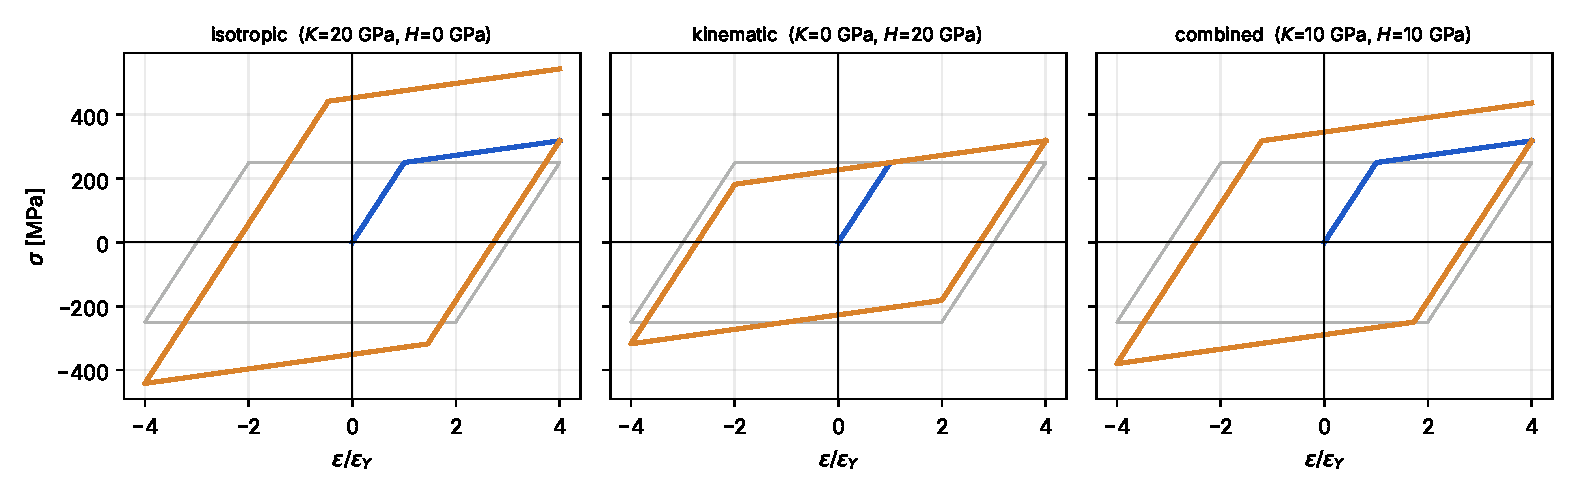
\includegraphics[width=\textwidth]{figures/ch4/filament_cycles.pdf}
\caption{Response of the filament to the strain cycle
$0\to4\varepsilon_Y\to-4\varepsilon_Y\to4\varepsilon_Y$,
$\varepsilon_Y=\sY/E$, with $E=200$\,GPa, $\sY=250$\,MPa and the same
monotonic curve, $K+H=20$\,GPa (a large value, chosen for legibility). Blue:
first loading; orange: the two reversals. Isotropic hardening (left) enlarges
the elastic range at each reversal; kinematic hardening (centre) translates
it, with early reverse yielding and a closed loop; combined hardening (right)
does both. The thin grey line is the perfectly plastic response.}
\label{fig:pl-cycles}
\end{figure}

\subsection{Energy and dissipation}\label{ssec:pl-1d-energy}
\index{dissipation!plastic}\index{energy!stored}%
The work supplied to the filament per unit volume, $\sigma\dot\varepsilon$, is
split into a stored part and a dissipated part. In the combined model, the
stored (free) energy is the elastic energy of the spring plus the energy of
two hardening springs,
\begin{equation}\label{eq:pl-1d-psi}
  \psi=\tfrac12E(\varepsilon-\varepsilon^p)^2+\tfrac12K\alpha^2+\tfrac12H\xi^2,
  \qquad \xi=\varepsilon^p\ \text{(kinematic variable)},\quad q=H\xi .
\end{equation}
Then $\dot\psi=\sigma(\dot\varepsilon-\dot\varepsilon^p)+K\alpha\dot\alpha+q\dot\varepsilon^p$
and the dissipation is
\begin{equation}\label{eq:pl-1d-diss}
  \mathcal D=\sigma\dot\varepsilon-\dot\psi=(\sigma-q)\dot\varepsilon^p-K\alpha\dot\alpha
  =\gamma\bigl(|\sigma-q|-K\alpha\bigr)=\sY\,\gamma=\sY\,\dot\alpha\ \ge0 ,
\end{equation}
where $|\sigma-q|=\sY+K\alpha$ was used, since $\gamma\ne0$ only on the yield
surface. The dissipation is the work of the friction element: its threshold
times its slip rate. The hardening springs store energy. This energy is given
back when the plastic strain is reversed in kinematic hardening; in isotropic
hardening it is never given back by the model (in metals it is the energy
stored in the dislocation structure).

\paragraph{Maximum dissipation in one dimension.}
\index{maximum plastic dissipation!one-dimensional}%
The flow rule of the perfectly plastic filament has a variational
characterization, which is the seed of Section~\ref{sec:pl-maxdiss}.
\begin{proposition}\label{prop:pl-1d-maxdiss}
Let $\Esig=[-\sY,\sY]$ and $\sigma\in\Esig$. The flow
rule~\eqref{eq:pl-1d-flow}--\eqref{eq:pl-1d-kt} holds if and only if
\[
  \sigma\,\dot\varepsilon^p\ \ge\ \sigma^\ast\,\dot\varepsilon^p\qquad\text{for all }\sigma^\ast\in\Esig .
\]
Among all admissible stresses, the actual stress maximizes the dissipated
power $\sigma^\ast\dot\varepsilon^p$, and the maximum is
$\sY|\dot\varepsilon^p|$.
\end{proposition}
\begin{proof}
If $|\sigma|<\sY$, the linear function $\sigma^\ast\mapsto\sigma^\ast\dot\varepsilon^p$ is
maximal at an interior point only if $\dot\varepsilon^p=0$; conversely the
flow rule gives $\gamma=0$. If $\sigma=\pm\sY$, the function is maximal on
$[-\sY,\sY]$ at $\pm\sY$ if and only if $\pm\dot\varepsilon^p\ge0$, that is
$\dot\varepsilon^p=\gamma\sign\sigma$ with $\gamma\ge0$.
\end{proof}

\subsection{The viscoplastic filament}\label{ssec:pl-vp1d}
\index{viscoplasticity!Perzyna}\index{viscoplasticity!filament}%
In viscoplasticity the stress may leave the elastic domain, and the plastic
strain rate depends on the distance to it, the \emph{overstress}. In the model
of Perzyna~\cite{Perzyna1966}, a dashpot of viscosity $\eta$ is placed in
parallel with the friction element, and the multiplier is given explicitly
instead of by the Kuhn--Tucker conditions:
\begin{equation}\label{eq:pl-perzyna1d}
  \sigma=E(\varepsilon-\varepsilon^{vp}),\qquad
  \dot\varepsilon^{vp}=\gamma\,\sign(\sigma),\qquad
  \gamma=\frac{\mac{f(\sigma)}}{\eta}=\frac{\mac{|\sigma|-\sY}}{\eta}.
\end{equation}
With the relaxation time $\tau=\eta/E$, and in a stress state outside the
elastic domain ($\sigma>\sY$, say), the evolution reads
\begin{equation}\label{eq:pl-perzyna-ode}
  \dot\sigma+\frac1\tau\,(\sigma-\sY)=E\dot\varepsilon .
\end{equation}
This is a linear ordinary differential equation, to which the standard
integration methods apply. In a relaxation test (strain held at
$\varepsilon_0>\sY/E$ from $t=0$), its solution is
\begin{equation}\label{eq:pl-relax}
  \sigma(t)=\sY+(E\varepsilon_0-\sY)\,e^{-t/\tau}\ \longrightarrow\ \sY\quad(t\to\infty).
\end{equation}
The stress relaxes to the yield surface. With $P\sigma=\sY\sign(\sigma)$ the
projection of $\sigma$ onto $\Esig$ when $|\sigma|>\sY$, the flow rule can be
written
\begin{equation}\label{eq:pl-dl1d}
  \dot\varepsilon^{vp}=\frac{1}{\tau E}\,(\sigma-P\sigma),
\end{equation}
which is the form of Duvaut and Lions~\cite{DuvautLions1972}. As
$\eta\to0$ the overstress vanishes and the rate-independent model is
recovered: viscoplasticity is a regularization (a penalty) of
plasticity~\cite[Sec.~1.6]{SimoHughes1998}.

%======================================================================
\section{Three-dimensional plasticity}\label{sec:pl-3d}
\index{plasticity!three-dimensional}%
The filament model extends to a three-dimensional body in small strains with
the same four ingredients. Stresses and strains are now symmetric
second-order tensors, elements of the space $\Sym$, and the plastic strain
$\epsp$ is a symmetric tensor field.

\subsection{Elastic law}\label{ssec:pl-elastic}
\index{plastic strain}\index{strain!additive decomposition}%
The strain is split additively, $\eps=\epse+\epsp$, and the stress is given by
the elastic law of Chapter~\ref{ch:elliptic} applied to the elastic part:
\begin{equation}\label{eq:pl-elastic}
  \sig=\bbC:(\eps-\epsp),\qquad
  \bbC=\kappa\,\tI\otimes\tI+2\mu\,\bbIdev\quad\text{(isotropy)},
\end{equation}
with the bulk modulus $\kappa$, the shear modulus $\mu$, and
$\bbIdev=\bbI-\tfrac13\tI\otimes\tI$ the projector onto deviatoric tensors.
For a given field $\epsp$, the plastic strain enters the equations exactly as
the thermal strain $\talpha\,\theta^D$ of Section~\ref{sec:el-energy}: it is an
\emph{initial strain} (an eigenstrain). The difference is that $\epsp$ is not
prescribed: it is an unknown, governed by an evolution law.

\subsection{Elastic domain and yield criteria}\label{ssec:pl-criteria}
\index{yield criterion}\index{elastic domain}\index{yield function}%
The elastic domain is a set of stresses and stress-like hardening variables
$\vq\in\R^m$, defined by a yield function:
\begin{equation}\label{eq:pl-domain}
  \Esig=\bigl\{(\sig,\vq)\in\Sym\times\R^m\ :\ f(\sig,\vq)\le0\bigr\}.
\end{equation}
Its interior $\{f<0\}$ is the set of elastic states, its boundary $\{f=0\}$
the yield surface. Outside $\Esig$ there are no admissible states. The
hardening variables $\vq$ describe the position and the size of the domain;
we first consider fixed $\vq$ and write $f(\sig)$.

\paragraph{Isotropy and invariants.}
\index{stress!invariants}\index{stress!deviator}\index{Haigh--Westergaard space}%
For an isotropic material, $f(\sig)$ depends only on the principal stresses
$\sigma_1,\sigma_2,\sigma_3$, symmetrically. It is convenient to split the
stress into its mean (hydrostatic) part and its deviator,
\[
  \sig=p\,\tI+\tens{s},\qquad p=\tfrac13\tr\sig,\qquad
  \tens{s}=\dev\sig=\sig-\tfrac13(\tr\sig)\,\tI,
\]
and to use the invariants $p$, $J_2=\tfrac12\tens{s}:\tens{s}$ and
$J_3=\det\tens{s}$. In the space of principal stresses, the hydrostatic axis
$\sigma_1=\sigma_2=\sigma_3$ carries $p$, and the plane orthogonal to it
through the origin (the \emph{deviatoric} or $\pi$-plane) carries $\tens{s}$.
In the $\pi$-plane, the deviator has polar coordinates $(\norm{\tens{s}},\theta)$,
where $\norm{\tens{s}}=\sqrt{\tens{s}:\tens{s}}=\sqrt{2J_2}$ and the Lode
angle $\theta$ is a function of $J_3/J_2^{3/2}$.

\paragraph{Metals are insensitive to pressure.} Plastic flow in metals is
produced by slip on crystallographic planes, driven by shear stresses. A
superposed hydrostatic pressure does not change the yield stress, and the
plastic strain is isochoric, $\tr\epsp=0$. The yield function then depends
on the deviator only, and the yield surface is a cylinder parallel to the
hydrostatic axis, described by its section in the $\pi$-plane
(Figure~\ref{fig:pl-loci}).

\begin{gbox}{Von Mises and Tresca criteria}
\index{von Mises criterion}\index{Tresca criterion}\index{equivalent stress}%
\begin{itemize}
  \item \emph{von Mises}: the elastic energy of distortion is bounded,
  \begin{equation}\label{eq:pl-mises}
    f(\sig)=\norm{\dev\sig}-\sqrt{\tfrac23}\,\sY\le0
    \quad\Longleftrightarrow\quad
    \sigma_{eq}=\sqrt{\tfrac32\,\dev\sig:\dev\sig}\le\sY .
  \end{equation}
  \item \emph{Tresca}: the maximal shear stress is bounded,
  \begin{equation}\label{eq:pl-tresca}
    f(\sig)=\max_{i,j}|\sigma_i-\sigma_j|-\sY\le0 .
  \end{equation}
\end{itemize}
Both are calibrated on the uniaxial tensile test: $\sig=\sigma\,\ve_1\otimes\ve_1$
yields at $|\sigma|=\sY$. In the $\pi$-plane the von Mises section is a circle
of radius $\sqrt{2/3}\,\sY$, and the Tresca section the regular hexagon
inscribed in it.
\end{gbox}

The two criteria differ most in shear. In tension--torsion,
$\sig=\sigma(\ve_1\otimes\ve_1)+\tau(\ve_1\otimes\ve_2+\ve_2\otimes\ve_1)$, they read
\begin{equation}\label{eq:pl-tt}
  \text{von Mises: }\ \sigma^2+3\tau^2\le\sY^2,\qquad
  \text{Tresca: }\ \sigma^2+4\tau^2\le\sY^2 ,
\end{equation}
so that the shear yield stress is $\sY/\sqrt3\approx0.577\,\sY$ for von Mises
and $\sY/2$ for Tresca. Tension--torsion experiments on most metals fall
between the two curves, closer to von Mises~\cite{Lubliner1990}.

\begin{figure}[h]
\centering
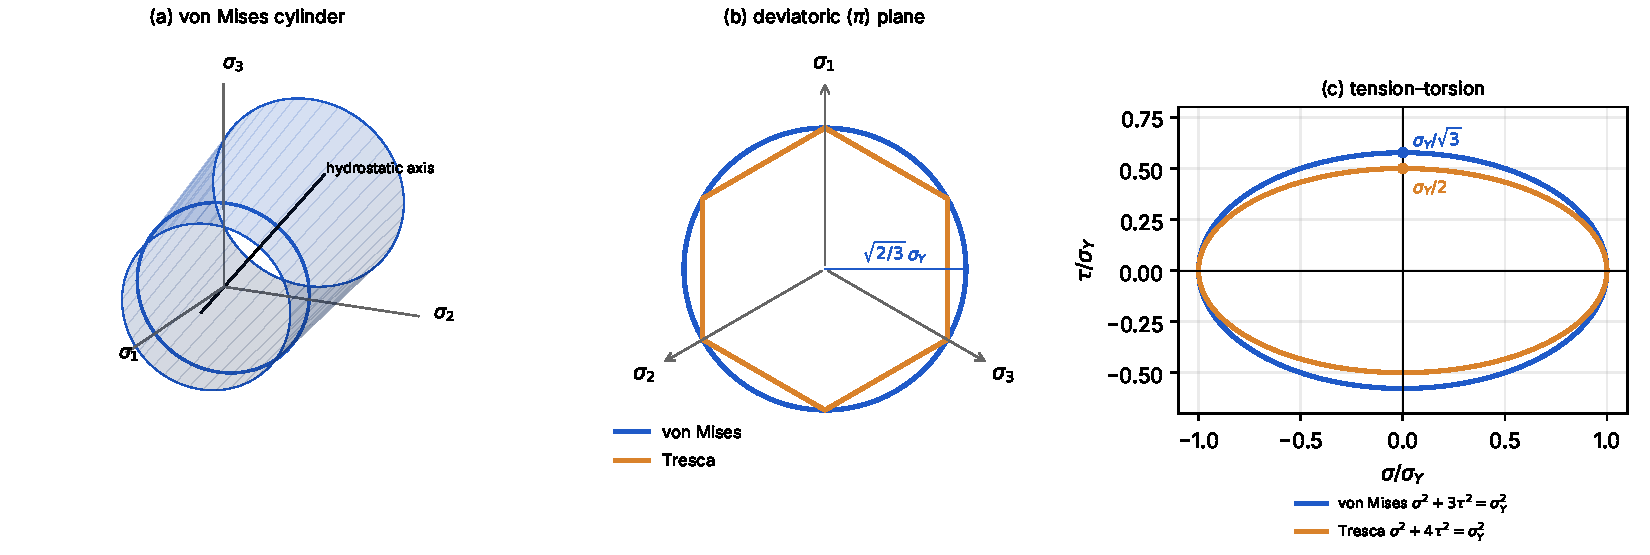
\includegraphics[width=\textwidth]{figures/ch4/yield_loci.pdf}
\caption{Left: sections of the von Mises cylinder (circle) and of the Tresca
prism (hexagon) by the $\pi$-plane; the projections of the principal axes are
drawn at $120^\circ$. Right: the same criteria in the tension--torsion plane
$(\sigma,\tau)$, ellipses~\eqref{eq:pl-tt}; the two coincide in pure tension
and differ most in pure shear.}
\label{fig:pl-loci}
\end{figure}

\paragraph{Pressure-sensitive materials.}
\index{Drucker--Prager criterion}\index{Mohr--Coulomb criterion}%
Soils, concrete, rocks and polymers are sensitive to pressure: confinement
raises their strength. The \emph{Drucker--Prager} criterion
$f(\sig)=\sigma_{eq}+\alpha_{DP}\tr\sig-\sigma_0\le0$ is a cone around the
hydrostatic axis, and the \emph{Mohr--Coulomb} criterion
$f(\sig)=(\sigma_1-\sigma_3)+(\sigma_1+\sigma_3)\sin\phi-2c\cos\phi\le0$
($\sigma_1\ge\sigma_2\ge\sigma_3$, friction angle $\phi$, cohesion $c$) a
hexagonal pyramid~\cite{Salencon2002}. All the criteria above define convex
sets; Section~\ref{sec:pl-maxdiss} explains why convexity is not an accident.

\subsection{Flow rule, hardening rule and loading conditions}\label{ssec:pl-flow}
\index{flow rule}\index{hardening rule}\index{flow rule!associative}%
The general model of rate-independent plasticity~\cite[Sec.~2.2]{SimoHughes1998}
gives the rates of the plastic strain and of the hardening variables in terms
of a single multiplier $\gamma$.
\begin{gbox}{Rate-independent plasticity}
\begin{align}
  &\sig=\bbC:(\eps-\epsp) && \text{elastic law},\label{eq:pl-box-el}\\
  &\Esig=\{(\sig,\vq)\ :\ f(\sig,\vq)\le0\} && \text{elastic domain},\label{eq:pl-box-dom}\\
  &\dot\eps^p=\gamma\,\tens{r}(\sig,\vq),\qquad \dot\vq=-\gamma\,\bbD\,\vect{h}(\sig,\vq)
  && \text{flow and hardening rules},\label{eq:pl-box-flow}\\
  &\gamma\ge0,\quad f(\sig,\vq)\le0,\quad\gamma\,f(\sig,\vq)=0 && \text{Kuhn--Tucker conditions},\label{eq:pl-box-kt}\\
  &\gamma\,\dot f(\sig,\vq)=0 && \text{consistency condition}.\label{eq:pl-box-cons}
\end{align}
The flow is \emph{associative} when the directions are the gradients of the
yield function: $\tens r=\partial_{\sig}f$, $\vect h=\partial_{\vq}f$.
\end{gbox}
\noindent Here $\bbD$ is a symmetric positive definite matrix of
\emph{hardening moduli} (generalized plastic moduli). In the associative case
the plastic strain rate is normal to the yield surface: this is the
\emph{normality rule}. The four cases of loading and unloading of the
filament hold without change, because they rest only on the following
property.

\begin{lemma}[Persistency]\label{lem:pl-persist}
For a piecewise smooth process with $f(\sig(t),\vq(t))\le0$ for all $t$, the
condition $f(t)=0$ implies $\dot f(t)\le0$, where $\dot f$ is the right time
derivative.
\end{lemma}
\begin{proof}
For $\Delta t>0$, $f(t+\Delta t)\le0=f(t)$. Dividing by $\Delta t$ and letting
$\Delta t\to0$ gives $\dot f(t)\le0$.
\end{proof}

\subsection{The plastic multiplier and the continuum tangent}\label{ssec:pl-tangent}
\index{plastic multiplier}\index{tangent modulus!continuum elastoplastic}%
Let the state be on the yield surface, $f(\sig,\vq)=0$, and the strain rate
$\dot\eps$ be given. Write $\partial_{\sig}f$ and $\partial_{\vq}f$ for the
gradients at the current state. By the chain rule and~\eqref{eq:pl-box-flow},
\begin{equation}\label{eq:pl-fdot}
  \dot f=\partial_{\sig}f:\dot\sig+\partial_{\vq}f\cdot\dot\vq
  =\partial_{\sig}f:\bbC:\dot\eps
  -\gamma\,\bigl(\partial_{\sig}f:\bbC:\tens r+\partial_{\vq}f\cdot\bbD\,\vect h\bigr).
\end{equation}
\begin{proposition}[Plastic multiplier and continuum tangent]\label{prop:pl-cep}
Assume that the \emph{hardening modulus}
$h_p=\partial_{\sig}f:\bbC:\tens r+\partial_{\vq}f\cdot\bbD\,\vect h$ is
positive. Then the Kuhn--Tucker and consistency conditions determine
\begin{equation}\label{eq:pl-gamma}
  \gamma=\frac{\mac{\partial_{\sig}f:\bbC:\dot\eps}}{h_p},
\end{equation}
and the stress rate is $\dot\sig=\bbC:\dot\eps$ if $\gamma=0$, and
$\dot\sig=\bbCep:\dot\eps$ if $\gamma>0$, with
\begin{equation}\label{eq:pl-cep}
  \bbCep=\bbC-\frac{(\bbC:\tens r)\otimes(\bbC:\partial_{\sig}f)}{h_p}.
\end{equation}
The continuum tangent $\bbCep$ is symmetric if the flow is associative.
\end{proposition}
\begin{proof}
If $\partial_{\sig}f:\bbC:\dot\eps<0$, then by~\eqref{eq:pl-fdot}
$\dot f<0$ for every $\gamma\ge0$, and consistency gives $\gamma=0$. If
$\partial_{\sig}f:\bbC:\dot\eps>0$, then $\gamma=0$ would give $\dot f>0$,
which Lemma~\ref{lem:pl-persist} excludes; hence $\gamma>0$, $\dot f=0$, and
$\gamma=\partial_{\sig}f:\bbC:\dot\eps/h_p$. The neutral case gives
$\gamma=0$. Then
$\dot\sig=\bbC:(\dot\eps-\gamma\,\tens r)=\bbC:\dot\eps-(\bbC:\tens r)\,
(\bbC:\partial_{\sig}f:\dot\eps)/h_p$, using the major symmetry of $\bbC$.
If $\tens r=\partial_{\sig}f$ the two vectors of the dyad coincide.
\end{proof}
The quantity $\partial_{\sig}f:\bbC:\dot\eps$ is the rate of $f$ produced by a
purely elastic response, $\dot f^\trial$, with the trial stress rate
$\dot\sig^\trial=\bbC:\dot\eps$. Geometrically, the material loads plastically
when $\dot\sig^\trial$ points out of the elastic domain, and unloads when it
points inwards (Figure~\ref{fig:pl-loading}). The loading criterion
$\dot f^\trial>0$ is written in terms of the strain rate, which is the
quantity controlled in a finite element computation.

\begin{figure}[h]
\centering
\begin{tikzpicture}[scale=1.0,>=Latex]
  \fill[cu!10,rotate=30] (0,0) ellipse (2.4 and 1.4);
  \draw[thick,cu,rotate=30] (0,0) ellipse (2.4 and 1.4);
  \node[cu] at (-0.6,0.0) {$\Esig\ (f<0)$};
  \node[cu] at (-1.6,2.3) {$\partial\Esig\ (f=0)$};
  \node[gray] at (3.9,-1.6) {$f>0$: not admissible};
  % boundary point: ellipse x=2.4cos t, y=1.4 sin t, t=-35deg, rotated 30
  \coordinate (P) at ({2.4*cos(-35)*cos(30)-1.4*sin(-35)*sin(30)},{2.4*cos(-35)*sin(30)+1.4*sin(-35)*cos(30)});
  % outward normal direction ~ (cos t/2.4, sin t/1.4) rotated
  \coordinate (N) at ($(P)+({0.83*(cos(-35)/2.4*cos(30)-sin(-35)/1.4*sin(30))*2.2},{0.83*(cos(-35)/2.4*sin(30)+sin(-35)/1.4*cos(30))*2.2})$);
  \draw[->,very thick] (P) -- (N) node[below right] {$\partial_{\sig}f$};
  % tangent line
  \draw[dashed,gray] ($(P)!2.2cm!90:(N)$) -- ($(P)!-2.0cm!90:(N)$);
  \draw[->,very thick,orange!80!black] (P) -- ++(1.6,0.9) node[right] {$\dot\sig^\trial=\bbC:\dot\eps$\ \ (loading)};
  \draw[->,very thick,cphi] (P) -- ++(-1.0,0.75) node[above left] {unloading};
  \fill (P) circle (1.6pt) node[left] {$(\sig,\vq)\ $};
\end{tikzpicture}
\caption{Loading and unloading, after Simo and
Hughes~\cite[Fig.~2-4]{SimoHughes1998}. At a point of the yield surface the
material loads plastically if the trial stress rate $\bbC:\dot\eps$ points to
the outside of the tangent plane (dashed), $\partial_{\sig}f:\bbC:\dot\eps>0$,
and unloads elastically if it points to the inside.}
\label{fig:pl-loading}
\end{figure}
The criterion $\dot f^\trial>0$ stays valid for softening materials, as long as $h_p>0$, whereas a criterion on the stress
rate would not. For a non-associative flow ($\tens r\ne\partial_{\sig}f$, as
for many soils), $\bbCep$ is not symmetric, and the tangent stiffness matrix
of a finite element computation is not symmetric either.

\subsection{\texorpdfstring{$J_2$}{J2} flow theory}\label{ssec:pl-j2}
\index{J2 flow theory@$J_2$ flow theory}\index{von Mises criterion!with hardening}\index{equivalent plastic strain}%
The model most used for metals combines the von Mises criterion with
isotropic and kinematic hardening and the associative flow
rule~\cite[Sec.~2.3.2]{SimoHughes1998}. Let $\tbeta$ be the back stress, a
deviatoric tensor (the centre of the von Mises cylinder), and $\alpha$ the
equivalent plastic strain. With the relative stress $\teta=\dev\sig-\tbeta$
and the unit normal $\tn=\teta/\norm{\teta}$,
\begin{gbox}{$J_2$ plasticity with linear isotropic and kinematic hardening}
\begin{align}
  &f(\sig,\tbeta,\alpha)=\norm{\dev\sig-\tbeta}-\sqrt{\tfrac23}\,(\sY+K\alpha),\label{eq:pl-j2-f}\\
  &\dot\eps^p=\gamma\,\tn,\qquad
  \dot{\tbeta}=\tfrac23H\,\gamma\,\tn,\qquad
  \dot\alpha=\sqrt{\tfrac23}\,\gamma ,\label{eq:pl-j2-flow}\\
  &\gamma=\frac{\mac{\tn:\dot\eps}}{1+\dfrac{K+H}{3\mu}},\qquad
  \bbCep=\kappa\,\tI\otimes\tI+2\mu\Bigl[\bbIdev-\frac{\tn\otimes\tn}{1+\dfrac{K+H}{3\mu}}\Bigr]
  \quad(\gamma>0).\label{eq:pl-j2-cep}
\end{align}
\end{gbox}
\noindent The plastic strain rate is deviatoric (isochoric flow), and
$\dot\alpha=\sqrt{2/3}\,\norm{\dot\eps^p}$. The factor $\sqrt{2/3}$ makes $\alpha$
equal to $|\varepsilon^p_{11}|$ in uniaxial tension, where
$\dot\eps^p=\dot\varepsilon^p_{11}\,\diag(1,-\tfrac12,-\tfrac12)$. To derive
the multiplier, note that $\tn$ is deviatoric and unitary, so that
$\tn:\dev\dot\sig=2\mu\,\tn:(\dot\eps-\gamma\tn)=2\mu\,\tn:\dot\eps-2\mu\gamma$, and
\[
  \dot f=\tn:(\dev\dot\sig-\dot{\tbeta})-\sqrt{\tfrac23}K\dot\alpha
  =2\mu\,\tn:\dot\eps-\gamma\bigl(2\mu+\tfrac23H+\tfrac23K\bigr).
\]
This is~\eqref{eq:pl-gamma} with $h_p=2\mu+\tfrac23(K+H)$; the tangent follows
from~\eqref{eq:pl-cep} with $\bbC:\tn=2\mu\tn$. For perfect plasticity
($K=H=0$), $\bbCep=\kappa\,\tI\otimes\tI+2\mu(\bbIdev-\tn\otimes\tn)$: the
stiffness in the direction $\tn$ vanishes.

In uniaxial stress the model reduces to the filament of
Section~\ref{ssec:pl-1d-kin}, with the same $K$ and $H$ and the back stress
$q=\tfrac32\beta_{11}=H\varepsilon^p_{11}$ (Exercise~\ref{exo:pl-uniaxial}).
In three dimensions, Simo and Hughes reserve the letter $\vq$ for the vector of
all stress-like hardening variables; for $J_2$ plasticity
$\vq=(-K\alpha,\,-\tbeta)$, $\bbD=\diag(K,\tfrac23H\,\bbI)$, and
\[
  f(\sig,\vq)=\norm{\dev\sig+\vq_{\mathrm{kin}}}-\sqrt{\tfrac23}\,(\sY-q_{\mathrm{iso}}),
\]
so that the associative rules $\dot\vq=-\gamma\,\bbD\,\partial_{\vq}f$
of~\eqref{eq:pl-box-flow} give back~\eqref{eq:pl-j2-flow}.

In the space of stresses, isotropic hardening expands the von Mises cylinder
and kinematic hardening translates it along the direction of plastic flow
(Figure~\ref{fig:pl-hardening}). Measured yield surfaces of metals after
plastic loading show both effects, with a translation that dominates at small
offsets~\cite{Lubliner1990}.

\begin{figure}[h]
\centering
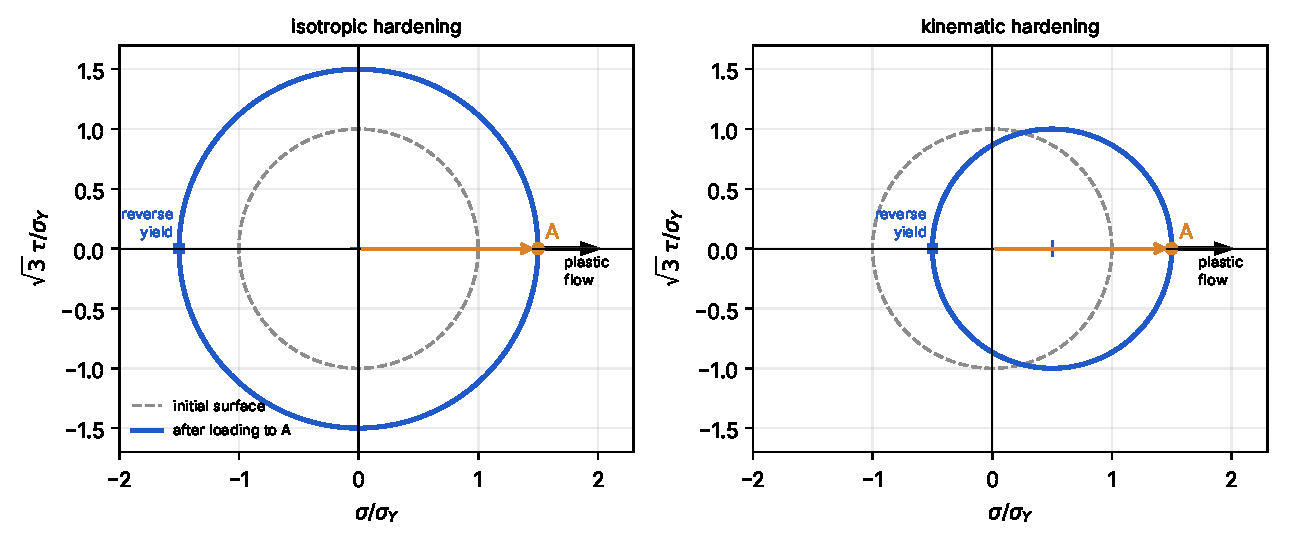
\includegraphics[width=0.85\textwidth]{figures/ch4/hardening_surfaces.pdf}
\caption{Section of the von Mises surface by the tension--torsion plane
$(\sigma,\sqrt3\tau)$, before (dashed) and after a tensile loading up to
$A=1.5\,\sY$. Isotropic hardening (left) expands the surface around the
origin; kinematic hardening (right) translates it, and reverse yielding in
compression starts at $\sigma=-0.5\,\sY$ instead of $-1.5\,\sY$
(Bauschinger effect). The plastic strain rate at $A$ is normal to the
surface.}
\label{fig:pl-hardening}
\end{figure}

\paragraph{Nonlinear hardening.}
\index{hardening!nonlinear}\index{Armstrong--Frederick model}\index{Voce law}%
Linear hardening is an approximation. Saturating laws are more realistic: the
\emph{Voce} law replaces $\sY+K\alpha$ by
$R(\alpha)=\sigma_\infty-(\sigma_\infty-\sY)e^{-\delta\alpha}$, and the
\emph{Armstrong--Frederick} law~\cite{ArmstrongFrederick1966} adds a recall
term to the kinematic rule, $\dot{\tbeta}=\tfrac23H\dot\eps^p-\zeta\,\tbeta\,\dot\alpha$,
which bounds the back stress. Formulas~\eqref{eq:pl-j2-cep} hold with $K$
replaced by $R'(\alpha)$ and $H$ by an effective modulus. The
Armstrong--Frederick law is not associative: the flow derives from a
pseudo-potential $F\ne f$~\cite{LemaitreChaboche1990}. It is therefore not a
generalized standard material in the sense of Section~\ref{sec:pl-gsm}, and
the results of Section~\ref{sec:pl-maxdiss} do not apply to it, although its
dissipation is non-negative (Exercise~\ref{exo:pl-af}).

\paragraph{Corners.}
\index{Tresca criterion!flow rule}\index{yield surface!corner}%
The Tresca criterion is not differentiable on the edges of the hexagon. It is
the intersection of six smooth (planar) criteria $f_\beta\le0$, and the flow
rule is then written with one multiplier per active surface,
$\dot\eps^p=\sum_\beta\gamma_\beta\,\partial_{\sig}f_\beta$ with
$\gamma_\beta\ge0$, $f_\beta\le0$, $\gamma_\beta f_\beta=0$ (Koiter's
rule~\cite{Koiter1953}). At a corner the flow direction can be any
combination of the normals of the adjacent faces: it lies in the cone of
normals. Section~\ref{sec:pl-maxdiss} gives this rule a single expression.

%======================================================================
\section{Thermodynamics and generalized standard materials}\label{sec:pl-gsm}
\index{generalized standard material}\index{thermodynamics!of plasticity}%
The model of Section~\ref{sec:pl-3d} was written as a list of rules. Halphen
and Nguyen~\cite{HalphenNguyen1975} showed that, for a large class of
materials, these rules follow from two convex functions: a free energy, which
gives the state laws, and a dissipation potential, which gives the evolution
laws. This structure, the one of \emph{generalized standard materials}
(GSM), guarantees the second principle of thermodynamics and is the source of
the variational principles and of the convergence properties used in this
chapter and the next two~\cite{GermainNguyenSuquet1983,LemaitreChaboche1990,Nguyen2000}.
We follow the presentation of Kondo and Maitournam~\cite{KondoMaitournam2023},
in the isothermal setting and in the notation of Simo and Hughes. The recipe
has three steps: choose the state variables; choose a free energy, which gives
the reversible part of the forces (the \emph{state laws}); choose a
dissipation potential, which gives their irreversible part (the
\emph{evolution laws}).

\subsection{State variables, state laws and dissipation}\label{ssec:pl-state}
\index{state laws}\index{free energy}\index{internal variables}\index{thermodynamic forces}%
The state of a material point is described by the total strain $\eps$ and by
internal variables $\vz=(\epsp,\valpha)$: the plastic strain and strain-like
hardening variables $\valpha\in\R^m$. The (Helmholtz) free energy per unit
volume, at fixed temperature, is
\begin{equation}\label{eq:pl-psi}
  \psi(\eps,\epsp,\valpha)=\tfrac12(\eps-\epsp):\bbC:(\eps-\epsp)+\psi_h(\valpha),
  \qquad\text{linear hardening: }\ \psi_h(\valpha)=\tfrac12\,\valpha\cdot\bbD\,\valpha .
\end{equation}
The \emph{state laws} define the stress and the \emph{thermodynamic forces}
conjugate to the internal variables:
\begin{equation}\label{eq:pl-statelaws}
  \sig=\frac{\partial\psi}{\partial\eps}=-\frac{\partial\psi}{\partial\epsp},
  \qquad
  \vq=-\frac{\partial\psi}{\partial\valpha}=-\bbD\,\valpha,
  \qquad
  \vSig:=-\frac{\partial\psi}{\partial\vz}=(\sig,\vq).
\end{equation}
The \emph{generalized stress} $\vSig$ collects the forces, and the
\emph{generalized plastic strain rate} $\dot\vz$ the fluxes, with the pairing
$\vSig\cdot\dot\vz=\sig:\dot\eps^p+\vq\cdot\dot\valpha$.

\paragraph{Clausius--Duhem inequality.}
\index{Clausius--Duhem inequality}\index{dissipation}%
In an isothermal process, the second principle requires that the intrinsic
dissipation, the power supplied minus the rate of free energy, be
non-negative. With the state laws,
\begin{equation}\label{eq:pl-CD}
  \mathcal D=\sig:\dot\eps-\dot\psi
  =\sig:\dot\eps-\frac{\partial\psi}{\partial\eps}:\dot\eps-\frac{\partial\psi}{\partial\vz}\cdot\dot\vz
  =\vSig\cdot\dot\vz=\sig:\dot\eps^p+\vq\cdot\dot\valpha\ \ge0 .
\end{equation}
The total strain is not a dissipative variable: the whole stress is
reversible, $\sig=\partial\psi/\partial\eps$, and the dissipation comes only
from the internal variables~\cite{KondoMaitournam2023}. (In a Kelvin--Voigt
viscoelastic solid, by contrast, the stress has an irreversible part.)
The dissipation is a product of forces and fluxes. In the language of Simo and
Hughes, the hardening rule $\dot\vq=-\gamma\bbD\,\partial_{\vq}f$ is the same as
$\dot\valpha=\gamma\,\partial_{\vq}f$, by~\eqref{eq:pl-statelaws}. The
associative model~\eqref{eq:pl-box-flow} therefore reads, in the generalized
variables,
\begin{equation}\label{eq:pl-assoc-gen}
  \dot\vz=\gamma\,\partial_{\vSig}f(\vSig),\qquad
  \gamma\ge0,\quad f(\vSig)\le0,\quad\gamma f(\vSig)=0 :
\end{equation}
the generalized plastic strain rate is normal to the elastic domain $\Esig$ in
the space of generalized stresses.

\paragraph{Example: $J_2$ plasticity.} The model~\eqref{eq:pl-j2-f}--\eqref{eq:pl-j2-flow}
has the internal variables $\valpha=(\alpha,\valpha_{\mathrm{kin}})$ with
$\valpha_{\mathrm{kin}}=\epsp$ (the kinematic variable follows the plastic
strain), the hardening energy and forces
\[
  \psi_h=\tfrac12K\alpha^2+\tfrac13H\,\epsp:\epsp,\qquad
  q_{\mathrm{iso}}=-K\alpha,\qquad \vq_{\mathrm{kin}}=-\tfrac23H\,\epsp=-\tbeta ,
\]
and the dissipation, computed as in~\eqref{eq:pl-1d-diss},
\begin{equation}\label{eq:pl-j2-diss}
  \mathcal D=\gamma\bigl(\tn:(\dev\sig-\tbeta)-\sqrt{\tfrac23}K\alpha\bigr)
  =\gamma\sqrt{\tfrac23}\,\bigl(\sY+K\alpha-K\alpha\bigr)=\sY\,\dot\alpha .
\end{equation}
As for the filament, only the initial yield stress dissipates; the hardening
part of the plastic work is stored.

\subsection{Generalized standard materials}\label{ssec:pl-gsm-def}
\index{dissipation potential}\index{generalized standard material!definition}\index{normality rule}%
\begin{definition}[Halphen--Nguyen~\cite{HalphenNguyen1975}]\label{def:pl-gsm}
A material is \emph{generalized standard} if its state laws derive from a free
energy $\psi(\eps,\vz)$, convex in $(\eps,\vz)$, and if there is a
\emph{dissipation potential} $\varphi(\dot\vz)$, convex, lower
semicontinuous, with $\varphi\ge0$ and $\varphi(\vzero)=0$, such that
\begin{equation}\label{eq:pl-normality}
  \vSig\in\partial\varphi(\dot\vz)
  \qquad\Longleftrightarrow\qquad
  \dot\vz\in\partial\varphi^\ast(\vSig).
\end{equation}
\end{definition}
\noindent The subdifferential $\partial\varphi$ is the set of slopes of the
supporting hyperplanes of $\varphi$ (it reduces to the gradient where
$\varphi$ is differentiable), and $\varphi^\ast$ is the Legendre--Fenchel
transform of $\varphi$ (Section~\ref{sec:var-dual}), the \emph{dual
dissipation potential}. The equivalence of the two forms
of~\eqref{eq:pl-normality} is the equality case of the Fenchel--Young
inequality. The first form, written as
$\vzero\in\partial_{\vz}\psi+\partial\varphi(\dot\vz)$, is a generalized Biot
equation; the second is the \emph{normality rule}.

\begin{proposition}\label{prop:pl-gsm-CD}
A generalized standard material satisfies the Clausius--Duhem inequality:
$\mathcal D=\vSig\cdot\dot\vz\ge\varphi(\dot\vz)\ge0$.
\end{proposition}
\begin{proof}
The subgradient inequality for $\varphi$ at $\dot\vz$, tested at $\vzero$,
gives $0=\varphi(\vzero)\ge\varphi(\dot\vz)+\vSig\cdot(\vzero-\dot\vz)$.
\end{proof}
A material defined by two convex potentials is thus thermodynamically
admissible \emph{for every process}: the second principle is built into the
structure. The modeller chooses $\psi$ and $\varphi$; no further check is
needed.

\paragraph{Rate independence and the elastic domain.}
\index{support function}\index{indicator function}\index{rate independence}%
Rate-independent plasticity corresponds to dissipation potentials that are
positively homogeneous of degree one: $\varphi(\lambda\dot\vz)=\lambda\,\varphi(\dot\vz)$
for $\lambda>0$.
\begin{proposition}\label{prop:pl-rateindep}
Let $\varphi\ge0$ be convex, lower semicontinuous and positively homogeneous of
degree one, and $\Esig=\partial\varphi(\vzero)=\{\vSig:\ \vSig\cdot\dot\vz\le\varphi(\dot\vz)\ \forall\dot\vz\}$.
Then $\Esig$ is closed and convex, contains $\vzero$, and
\[
  \varphi^\ast=I_{\Esig},\qquad
  \varphi(\dot\vz)=\pi_{\Esig}(\dot\vz):=\sup_{\vSig^\ast\in\Esig}\vSig^\ast\cdot\dot\vz ,
\]
where $I_{\Esig}$ is the indicator function of $\Esig$ ($0$ on $\Esig$,
$+\infty$ outside) and $\pi_{\Esig}$ its support function. Conversely,
every closed convex set containing $\vzero$ defines such a potential.
\end{proposition}
\begin{proof}
For a given $\vSig$, the function $\dot\vz\mapsto\vSig\cdot\dot\vz-\varphi(\dot\vz)$
is positively homogeneous. Either it is $\le0$ everywhere, and its supremum
$\varphi^\ast(\vSig)$ is $0$ (value at $\dot\vz=\vzero$); or it is positive
somewhere, and then $\varphi^\ast(\vSig)=+\infty$ by scaling. Hence
$\varphi^\ast=I_{\Esig}$ with $\Esig$ as stated. As $\varphi$ is convex and
lower semicontinuous, $\varphi=\varphi^{\ast\ast}=I_{\Esig}^\ast=\pi_{\Esig}$.
\end{proof}
The dual potential of a rate-independent material is the indicator of its
elastic domain, and the normality rule~\eqref{eq:pl-normality} becomes
$\dot\vz\in\partial I_{\Esig}(\vSig)$. Since $\partial\varphi(\lambda\dot\vz)=\partial\varphi(\dot\vz)$
for $\lambda>0$, a change of time scale leaves the evolution unchanged: this
is rate independence. The dissipation potential is the \emph{dissipation
function} $\pi_{\Esig}$: by Proposition~\ref{prop:pl-gsm-CD} and the
definition of $\Esig$, $\mathcal D=\pi_{\Esig}(\dot\vz)$ for the actual
process. For $J_2$ plasticity with isotropic hardening,
$\pi_{\Esig}(\dot\eps^p,\dot\alpha)=\sY\dot\alpha$ on the admissible rates
(Example~\ref{ex:pl-mises-pi}), in agreement
with~\eqref{eq:pl-j2-diss}.

\paragraph{Viscoplasticity.}
\index{viscoplasticity!dual potential}\index{Norton--Hoff law}\index{viscoplasticity!Duvaut--Lions}%
A smooth, finite dual potential gives a viscoplastic material. With a
viscosity $\eta$, or a reference strain rate $\dot\varepsilon_0$ and an
exponent $m$:
\begin{align}
  \text{Perzyna:}\quad&\varphi^\ast(\vSig)=\frac1{2\eta}\mac{f(\vSig)}^2,
  &&\dot\vz=\frac1\eta\,\mac{f(\vSig)}\,\partial_{\vSig}f,\label{eq:pl-perzyna}\\
  \text{Norton--Hoff:}\quad&\varphi^\ast(\sig)=\frac{\sigma_0\dot\varepsilon_0}{m+1}\,
  \Bigl\langle\frac{\sigma_{eq}-\sY}{\sigma_0}\Bigr\rangle^{m+1},
  &&\dot\eps^p=\dot\varepsilon_0\Bigl\langle\frac{\sigma_{eq}-\sY}{\sigma_0}\Bigr\rangle^{m}\,\frac32\,\frac{\dev\sig}{\sigma_{eq}} .\label{eq:pl-norton}
\end{align}
The Duvaut--Lions model~\cite{DuvautLions1972} uses the squared distance to
$\Esig$ instead, $\varphi^\ast=\tfrac{1}{2\tau}\,\mathrm{dist}_E^2(\vSig,\Esig)$,
measured in the energy norm~\eqref{eq:pl-energynorm} below, with a
relaxation time $\tau$. Its one-dimensional form is~\eqref{eq:pl-dl1d}. As
$\eta\to0$ (or $\tau\to0$) the Perzyna and Duvaut--Lions potentials tend to
$I_{\Esig}$: the rate-independent model is their limit.

\subsection{A dictionary}\label{ssec:pl-dictionary}
Simo and Hughes and the French school of Halphen, Nguyen, Germain and Suquet
describe the same model in two languages. Table~\ref{tab:pl-dictionary} gives
the correspondence used in this book.

\begin{table}[h]
\centering\small
\renewcommand{\arraystretch}{1.2}
\begin{tabular}{@{}lll@{}}
\toprule
 & \sffamily Simo--Hughes~\cite{SimoHughes1998} & \sffamily Halphen--Nguyen~\cite{HalphenNguyen1975}\\
\midrule
internal variables & $\epsp$, $\valpha$ & $\vz=(\epsp,\valpha)$\\
forces & $\sig$, $\vq=-\bbD\valpha$ & $\vSig=(\sig,\vq)=-\partial_{\vz}\psi$\\
elastic domain & $f(\sig,\vq)\le0$ & $\Esig=\partial\varphi(\vzero)$\\
flow rule & $\dot\eps^p=\gamma\,\partial_{\sig}f$, $\dot\vq=-\gamma\bbD\,\partial_{\vq}f$ & $\dot\vz\in\partial\varphi^\ast(\vSig)=\partial I_{\Esig}(\vSig)$\\
loading/unloading & Kuhn--Tucker, consistency & normal cone (Section~\ref{sec:pl-maxdiss})\\
dissipation & $\sig:\dot\eps^p+\vq\cdot\dot\valpha$ & $\varphi(\dot\vz)=\pi_{\Esig}(\dot\vz)$\\
principle & maximum plastic dissipation & normality, monotonicity\\
energy norm & $\sig:\bbS:\sig+\vq\cdot\bbD^{-1}\vq$ & same\\
\bottomrule
\end{tabular}
\caption{Simo--Hughes and generalized standard materials: one model, two
notations.}
\label{tab:pl-dictionary}
\end{table}

\paragraph{The complementary energy norm.}
\index{energy!complementary (plasticity)}%
The last line of the table defines a scalar product on generalized stresses,
\begin{equation}\label{eq:pl-energynorm}
  \scal{\vSig}{\vSig'}_{E}=\sig:\bbS:\sig'+\vq\cdot\bbD^{-1}\vq',\qquad
  \norm{\vSig}_E^2=\scal{\vSig}{\vSig}_E ,
\end{equation}
where $\tfrac12\norm{\vSig}_E^2$ is the complementary energy, elastic plus
hardening. Chapter~5 shows that the implicit integration of the
flow rule is the projection of a trial state onto $\Esig$ in this norm.

%======================================================================
\section{The principle of maximum plastic dissipation}\label{sec:pl-maxdiss}
\index{maximum plastic dissipation}%
The normality rule has a variational form, which extends
Proposition~\ref{prop:pl-1d-maxdiss}: among all admissible generalized
stresses, the actual one maximizes the dissipated power. It was postulated by
Hill~\cite{Hill1950}; it also follows from Drucker's stability
postulate~\cite{Drucker1951,Lubliner1990}. We first recall a few notions of
convex analysis~\cite{RockafellarConvex}.

\subsection{Normal cones}\label{ssec:pl-cones}
\index{normal cone}\index{subdifferential}%
Let $\mathcal K$ be a nonempty closed convex set in a space with scalar product
$\vx\cdot\vy$.
\begin{gbox}{Normal cone and support function}
\begin{itemize}
  \item The \emph{normal cone} to $\mathcal K$ at $\vx\in \mathcal K$ is the set of directions
  that make an obtuse angle with every chord from $\vx$:
  $N_{\mathcal K}(\vx)=\{\vy:\ \vy\cdot(\vx'-\vx)\le0\ \ \forall\vx'\in \mathcal K\}$. It is
  $\{\vzero\}$ at interior points, a half-line along the outward normal at a
  smooth boundary point, and a cone of normals at a corner.
  \item $N_{\mathcal K}(\vx)=\partial I_{\mathcal K}(\vx)$: the normal cone is the subdifferential
  of the indicator function.
  \item $I_{\mathcal K}^\ast=\pi_{\mathcal K}$, and by Fenchel--Young, for $\vx\in \mathcal K$:
  $\ \vy\in N_{\mathcal K}(\vx)\iff\vx\in\partial\pi_{\mathcal K}(\vy)\iff\vx\cdot\vy=\pi_{\mathcal K}(\vy)$.
  \item If $\mathcal K=\{f\le0\}$ with $f$ convex and differentiable and $f(\vx_0)<0$ for
  some $\vx_0$ (\emph{Slater condition}), then $N_{\mathcal K}(\vx)=\{\vzero\}$ if
  $f(\vx)<0$ and $N_{\mathcal K}(\vx)=\{\gamma\nabla f(\vx):\gamma\ge0\}$ if $f(\vx)=0$.
  For $\mathcal K=\bigcap_\beta\{f_\beta\le0\}$, $N_{\mathcal K}(\vx)$ is the set of combinations
  $\sum_\beta\gamma_\beta\nabla f_\beta(\vx)$ with $\gamma_\beta\ge0$ and
  $\gamma_\beta=0$ when $f_\beta(\vx)<0$.
\end{itemize}
\end{gbox}
The first three items follow from the definitions and from
Section~\ref{sec:var-dual}; the last one is proved
in~\cite[Sec.~23]{RockafellarConvex}.

\subsection{The principle and its equivalent forms}\label{ssec:pl-maxdiss-thm}
\begin{theorem}[Maximum plastic dissipation]\label{thm:pl-maxdiss}
Let $\Esig$ be closed and convex with $\vzero\in\Esig$, let $\vSig\in\Esig$ and
let $\dot\vz$ be a generalized plastic strain rate. The following are
equivalent.
\begin{enumerate}[label=(\alph*)]
  \item \emph{Maximum dissipation:} $\vSig\cdot\dot\vz\ge\vSig^\ast\cdot\dot\vz$
  for all $\vSig^\ast\in\Esig$.
  \item \emph{Normality:} $\dot\vz\in N_{\Esig}(\vSig)=\partial I_{\Esig}(\vSig)$.
  \item \emph{Generalized standard form:} $\vSig\in\partial\pi_{\Esig}(\dot\vz)$.
  \item \emph{Dissipation identity:} $\mathcal D=\vSig\cdot\dot\vz=\pi_{\Esig}(\dot\vz)$.
\end{enumerate}
If moreover $\Esig=\{f\le0\}$ with $f$ convex, differentiable and
$f(\vzero)<0$, they are equivalent to
\begin{enumerate}[label=(\alph*),start=5]
  \item \emph{associative flow rule and Kuhn--Tucker conditions:}
  $\dot\vz=\gamma\,\partial_{\vSig}f(\vSig)$, $\gamma\ge0$, $f(\vSig)\le0$,
  $\gamma f(\vSig)=0$.
\end{enumerate}
\end{theorem}
\begin{proof}
(a)$\iff$(b): (a) reads $\dot\vz\cdot(\vSig^\ast-\vSig)\le0$ for all
$\vSig^\ast\in\Esig$, the definition of the normal cone.
(b)$\iff$(c)$\iff$(d): third item of the box above, with $\mathcal K=\Esig$,
$\vx=\vSig$, $\vy=\dot\vz$.
(b)$\iff$(e): fourth item, with $\vx_0=\vzero$.
\end{proof}

\begin{figure}[h]
\centering
\begin{tikzpicture}[scale=1.05,>=Latex]
  \def\domain{(2.4,0) -- (1.6,1.5) .. controls (0.8,2.1) and (-0.6,2.1) .. (-1.5,1.4) .. controls (-2.3,0.8) and (-2.3,-0.8) .. (-1.5,-1.4) .. controls (-0.6,-2.1) and (0.8,-2.1) .. (1.6,-1.5) -- cycle}
  \fill[cu!10] \domain;
  \draw[thick,cu] \domain;
  \node[cu] at (-0.7,0.35) {$\Esig=\{f\le0\}$};
  \fill (-0.3,-0.9) circle (1.4pt) node[below] {$\vSig$: $N_{\Esig}=\{\vzero\}$};
  \coordinate (s) at (0.09,1.94);
  \fill (s) circle (1.4pt);
  \draw[->,very thick,orange!80!black] (s) -- (0.09,3.0) node[above] {$\dot\vz=\gamma\,\partial_{\vSig}f$};
  \draw[dashed,orange!80!black] (-1.7,1.94) -- (1.8,1.94);
  \node[orange!80!black,font=\small,above] at (-1.25,1.94) {supporting plane};
  \coordinate (c) at (2.4,0);
  \fill[orange!20] (c) -- ($(c)+(1.32,0.71)$) -- ($(c)+(1.32,-0.71)$) -- cycle;
  \draw[orange!80!black,thick] (c) -- ($(c)+(1.32,0.71)$);
  \draw[orange!80!black,thick] (c) -- ($(c)+(1.32,-0.71)$);
  \fill (c) circle (1.4pt);
  \node[orange!80!black,font=\small,right] at (3.75,0) {$N_{\Esig}(\vSig)$ (corner)};
\end{tikzpicture}
\caption{Geometry of the principle of maximum plastic dissipation. Inside the
elastic domain there is no plastic flow. At a smooth point of the yield
surface the flow is along the outward normal, and the plane orthogonal to
$\dot\vz$ through $\vSig$ supports $\Esig$. At a corner (Tresca) the flow
lies in the cone of normals.}
\label{fig:pl-normality}
\end{figure}

\begin{remark}[The Lagrangian of Simo and Hughes]\label{rem:pl-kkt}
\index{Karush--Kuhn--Tucker conditions!plasticity}%
Statement (a) is a constrained optimization problem: the actual $\vSig$
minimizes $-\vSig^\ast\cdot\dot\vz$ under the constraint $f(\vSig^\ast)\le0$.
Its Lagrangian is $\mathcal L(\vSig^\ast,\gamma)=-\vSig^\ast\cdot\dot\vz+\gamma f(\vSig^\ast)$,
and its Karush--Kuhn--Tucker conditions (Section~\ref{sec:var-lagrange}) are
statement (e): the plastic multiplier is the Lagrange multiplier of the yield
constraint~\cite[Sec.~2.6]{SimoHughes1998}. The Slater condition $f(\vzero)<0$
is the constraint qualification which guarantees that the multiplier exists.
\end{remark}

\subsection{Consequences}\label{ssec:pl-consequences}
\paragraph{Convexity of the elastic domain.}
\index{elastic domain!convexity}%
If the principle holds at every point of the yield surface for some
$\dot\vz\ne\vzero$, then through every boundary point passes a plane that
leaves $\Esig$ on one side (Figure~\ref{fig:pl-normality}). A closed set with
nonempty interior having this property is convex. Maximum dissipation
\emph{implies} the convexity of the elastic domain and the normality of the
flow~\cite{SimoHughes1998,Lubliner1990}. Measured yield surfaces of metals
are indeed convex, and the measured plastic strain rates close to normal.

\paragraph{Monotonicity.}
\index{monotonicity!of the flow rule}%
\begin{corollary}\label{cor:pl-monotone}
If $\dot\vz_1\in N_{\Esig}(\vSig_1)$ and $\dot\vz_2\in N_{\Esig}(\vSig_2)$, then
$(\vSig_1-\vSig_2)\cdot(\dot\vz_1-\dot\vz_2)\ge0$.
\end{corollary}
\begin{proof}
By (a), $\vSig_1\cdot\dot\vz_1\ge\vSig_2\cdot\dot\vz_1$ and
$\vSig_2\cdot\dot\vz_2\ge\vSig_1\cdot\dot\vz_2$. Add the two inequalities.
\end{proof}
The flow rule is a \emph{monotone} relation between forces and fluxes, the
nonlinear analogue of a positive definite matrix. Monotonicity is the
property behind the uniqueness of the stresses (Section~\ref{sec:pl-bvp}),
the stability of the integration algorithms (Chapter~5) and the
convergence of the global--local methods (Chapter~6).

\paragraph{The dissipation function of von Mises.}
\begin{example}\label{ex:pl-mises-pi}
\index{support function!von Mises}%
Take isotropic hardening, $\vz=(\epsp,\alpha)$, $q=-K\alpha$ and
$\Esig=\{(\sig,q):\ \norm{\dev\sig}-\sqrt{2/3}\,(\sY-q)\le0\}$. Then
\begin{equation}\label{eq:pl-mises-pi}
  \pi_{\Esig}(\dot\eps^p,\dot\alpha)=
  \begin{cases}\sY\,\dot\alpha & \text{if }\tr\dot\eps^p=0\text{ and }
  \dot\alpha\ge\sqrt{\tfrac23}\,\norm{\dot\eps^p},\\
  +\infty & \text{otherwise.}\end{cases}
\end{equation}
Indeed, write $\sig=p\tI+\tens s$. If $\tr\dot\eps^p\neq0$, letting
$p\to\pm\infty$ in $\sig:\dot\eps^p+q\dot\alpha$ gives $+\infty$. Otherwise, at
fixed $q\le\sY$, the supremum of $\tens s:\dot\eps^p$ over
$\norm{\tens s}\le\sqrt{2/3}\,(\sY-q)$ is $\sqrt{2/3}\,(\sY-q)\,\norm{\dot\eps^p}$,
so that
\[
  \pi_{\Esig}=\sqrt{\tfrac23}\,\sY\norm{\dot\eps^p}
  +\sup_{q\le\sY}\ q\Bigl(\dot\alpha-\sqrt{\tfrac23}\norm{\dot\eps^p}\Bigr).
\]
The supremum is $+\infty$ if the bracket is negative ($q\to-\infty$) and is
attained at $q=\sY$ otherwise, which gives $\sY\dot\alpha$. The infinite values
encode the constraints of the model: isochoric flow, and $\alpha$ at least the
accumulated equivalent plastic strain. The flow rule realizes the
constraint with equality, $\dot\alpha=\sqrt{2/3}\norm{\dot\eps^p}$. Without
hardening ($K=0$, only $\epsp$),
$\pi(\dot\eps^p)=\sqrt{2/3}\,\sY\norm{\dot\eps^p}$ on isochoric rates; this
function is used in limit analysis (Section~\ref{ssec:pl-limit}).
\end{example}

%======================================================================
\section{The elastoplastic boundary-value problem}\label{sec:pl-bvp}
\index{elastoplasticity!boundary-value problem}\index{quasi-static evolution}%
A body $\Omega$ made of an elastoplastic material is loaded by body forces
$\vfD(t)$, tractions $\vtD(t)$ on $S_t$ and displacements $\vuD(t)$ on $S_u$,
slowly enough for inertia to be negligible. Time $t\in[0,T]$ orders the
loading; for a rate-independent material only the path matters, not the
rate. The unknowns are the displacement $\vu(\vx,t)$, the stress $\sig(\vx,t)$
and the internal variables $\vz(\vx,t)=(\epsp,\valpha)(\vx,t)$.

\subsection{Equations}\label{ssec:pl-bvp-eq}
\begin{gbox}{Quasi-static elastoplastic evolution problem}
For $t\in[0,T]$:
\begin{align}
  &\eps=\tfrac12(\nabla\vu+\nabla\vu\T)\ \text{in }\Omega,\qquad \vu=\vuD(t)\ \text{on }S_u
  &&\text{kinematics},\label{eq:pl-bvp-kin}\\
  &\dive\sig+\vfD(t)=\vzero\ \text{in }\Omega,\qquad \sig\vn=\vtD(t)\ \text{on }S_t
  &&\text{equilibrium},\label{eq:pl-bvp-eq}\\
  &\sig=\bbC:(\eps-\epsp),\qquad \vq=-\bbD\,\valpha
  &&\text{state laws},\label{eq:pl-bvp-state}\\
  &\dot\vz\in N_{\Esig}(\vSig),\qquad \vSig=(\sig,\vq)\in\Esig
  &&\text{flow rule},\label{eq:pl-bvp-flow}
\end{align}
with initial conditions $\vz(\vx,0)=\vz_0(\vx)$, usually $\vz_0=\vzero$.
\end{gbox}
\noindent In weak form, equilibrium reads: $\vu(t)\in\Kad(\vuD(t),S_u)$ and
\begin{equation}\label{eq:pl-bvp-weak}
  \int_\Omega\sig(t):\eps[\vv]\dd x=\int_\Omega\vfD(t)\cdot\vv\dd x+\int_{S_t}\vtD(t)\cdot\vv\dd s
  \qquad\forall\vv\in\Kad(\vzero,S_u).
\end{equation}
The equations split into two groups of different nature
(Figure~\ref{fig:pl-tonti}). Kinematics, equilibrium and the state laws are
\emph{linear} and \emph{global}: at a given instant, and for a given field of
internal variables, they form a linear elasticity problem with initial strain
$\epsp$. The flow rule is \emph{nonlinear} and \emph{local}: it is an
evolution law at each material point, coupled to the others only through the
stress. Every algorithm of Chapters~5 and~6
exploits this split.

\begin{figure}[h]
\centering
\begin{tikzpicture}[node distance=1.15cm and 1.3cm]
  \node[smallbox,kin,minimum width=4.4cm] (u) {$\vu$, \quad $\vu=\vuD(t)$ on $S_u$\\ \footnotesize displacement};
  \node[smallbox,stat,minimum width=4.4cm,right=3.4cm of u] (f) {$\dive\sig+\vfD=\vzero$,\ \ $\sig\vn=\vtD$ on $S_t$\\ \footnotesize body forces and tractions};
  \node[smallbox,kin,minimum width=4.4cm,below=of u] (e) {$\eps[\vu]=\epse+\epsp$\\ \footnotesize strain};
  \node[smallbox,stat,minimum width=4.4cm,below=of f] (s) {$\sig=\bbC:\epse$, \ $(\sig,\vq)\in\Esig$\\ \footnotesize stress};
  \node[smallbox,key,minimum width=4.4cm,below=1.5cm of $(e)!0.5!(s)$] (z) {$\dot\vz\in N_{\Esig}(\sig,\vq)$\\ \footnotesize flow rule (local, nonlinear)};
  \draw[arr] (u) -- (e) node[midway,left,font=\small]{$\eps[\cdot]$};
  \draw[arr] (e) -- (s) node[midway,above,font=\small]{$\bbC$};
  \draw[arr] (s) -- (f) node[midway,right,font=\small]{$-\dive$, \ $\cdot\,\vn$};
  \draw[arr] (s.south) |- (z.east);
  \draw[arr] (z.west) -| (e.south) node[pos=0.75,left,font=\small]{$\epsp$};
  \node[below=0.12cm of e.south west,anchor=north west,kinlab] {$\Kad(\vuD,S_u)$};
  \node[below=0.12cm of s.south east,anchor=north east,statlab] {$\Sad(\vfD,\vtD,S_t)$};
\end{tikzpicture}
\caption{Tonti diagram of elastoplasticity. The upper part is the diagram of
linear elasticity (Figure~\ref{fig:tonti-el}), with the plastic strain as an
initial strain. The flow rule (orange) closes the loop: it is the only
nonlinear relation, and it is local.}
\label{fig:pl-tonti}
\end{figure}

\subsection{Uniqueness of the stresses}\label{ssec:pl-unique}
\index{uniqueness!elastoplastic stresses}%
\begin{theorem}\label{thm:pl-unique}
Let $(\vu_i,\sig_i,\vz_i)$, $i=1,2$, be two smooth solutions of the evolution
problem with the same data and the same initial state. Let $\bbC$ be
symmetric positive definite, and $\bbD$ symmetric positive definite on the
hardening variables present in the model. Then $\sig_1=\sig_2$ and
$\vq_1=\vq_2$ at all times. For $J_2$ plasticity with $K>0$ or $H>0$ (keeping
only the hardening variables whose modulus is positive) the
plastic strains, the strains and, if $S_u$ prevents rigid motions, the
displacements coincide too.
\end{theorem}
\begin{proof}
Write $\Delta(\cdot)=(\cdot)_1-(\cdot)_2$ and consider the complementary energy
of the difference,
$\displaystyle \mathcal E(t)=\frac12\int_\Omega\bigl(\Delta\sig:\bbS:\Delta\sig+\Delta\vq\cdot\bbD^{-1}\Delta\vq\bigr)\dd x$.
By the state laws, $\bbS:\Delta\dot\sig=\Delta\dot\eps-\Delta\dot\eps^p$ and
$\bbD^{-1}\Delta\dot\vq=-\Delta\dot\valpha$, so that
\[
  \dot{\mathcal E}=\int_\Omega\Delta\sig:\eps[\Delta\dot\vu]\dd x
  -\int_\Omega\bigl(\Delta\sig:\Delta\dot\eps^p+\Delta\vq\cdot\Delta\dot\valpha\bigr)\dd x .
\]
The first integral vanishes: $\Delta\dot\vu\in\Kad(\vzero,S_u)$, and
$\Delta\sig$ is self-equilibrated (zero body force, zero traction on $S_t$),
so the weak form~\eqref{eq:pl-bvp-weak} applies with $\vv=\Delta\dot\vu$. The
second integrand is $\Delta\vSig\cdot\Delta\dot\vz\ge0$ by
Corollary~\ref{cor:pl-monotone}. Hence $\dot{\mathcal E}\le0$; since
$\mathcal E(0)=0$ and $\mathcal E\ge0$, $\mathcal E\equiv0$. With hardening,
$\Delta\valpha=-\bbD^{-1}\Delta\vq=\vzero$. For $J_2$ plasticity this fixes the
plastic strain: with kinematic hardening $\epsp=\valpha_{\mathrm{kin}}$; with
isotropic hardening $\dot\eps^p=\gamma\tn$, where $\tn$ is given by the stress
and $\gamma=\sqrt{3/2}\,\dot\alpha$. Hence $\Delta\epsp=\vzero$ and
$\eps[\Delta\vu]=\bbS:\Delta\sig+\Delta\epsp=\vzero$, and $\Delta\vu$ is a rigid
motion vanishing on $S_u$.
\end{proof}
Without hardening the stresses are still unique. The plastic strains and the
displacements need not be: at the limit load, the body may flow along a
mechanism of arbitrary amplitude
(Example~\ref{ex:pl-bar}). The natural function space for perfect plasticity
is then not $H^1$ but the space $BD(\Omega)$ of displacements whose strain is a
bounded measure: the plastic strain may concentrate on surfaces (slip lines,
shear bands) and the displacement may jump across
them~\cite{Temam1983,HanReddy2013}.

\subsection{The rate problem: Hill's minimum principle}\label{ssec:pl-hill}
\index{Hill's minimum principle}\index{rate problem}%
At a given instant, with the current state known, the \emph{rate problem}
determines the rates $(\dot\vu,\dot\vz)$ from the load rates. At each point
where the state is on the yield surface, the rate of the plastic strain is
given by Proposition~\ref{prop:pl-cep} and depends on the sign of
$\partial_{\sig}f:\bbC:\eps[\dot\vu]$. The rate problem is therefore a
piecewise linear problem: it behaves as an elasticity problem with moduli
$\bbCep$ in the zones that load plastically and $\bbC$ elsewhere, but the
zones are unknown. Hill~\cite{Hill1958} showed that it is a minimization.

\begin{theorem}[Hill~\cite{Hill1958,Nguyen2000}]\label{thm:pl-hill}
Let the current state $(\sig,\vq)$ be given, with $\bbC$ and $\bbD$ symmetric
positive definite. Among the kinematically admissible velocity fields
$\vv\in\Kad(\dot\vuD,S_u)$ and the generalized plastic strain rates
$\vect{\zeta}(\vx)\in N_{\Esig}(\vSig(\vx))$, the solution of the rate problem
minimizes
\[
  \mathcal F(\vv,\vect\zeta)=\int_\Omega\Bigl[\tfrac12\bigl(\eps[\vv]-\vect\zeta_p\bigr):\bbC:\bigl(\eps[\vv]-\vect\zeta_p\bigr)
  +\tfrac12\,\vect\zeta_\alpha\cdot\bbD\,\vect\zeta_\alpha\Bigr]\dd x
  -\int_\Omega\dot\vfD\cdot\vv\dd x-\int_{S_t}\dot\vtD\cdot\vv\dd s ,
\]
where $\vect\zeta=(\vect\zeta_p,\vect\zeta_\alpha)$. The stress rates are unique.
\end{theorem}
\noindent The functional is the potential energy of the rates, with the
plastic strain rate as an unknown initial strain constrained to the normal
cone. The minimization in $\vect\zeta$ at fixed $\vv$ is local, and its
optimality condition is the consistency condition $\dot\vSig\cdot\vect\zeta=0$
with $\dot\vSig$ tangent to $\Esig$ (Exercise~\ref{exo:pl-hill1d}). The
functional is convex as long as $\bbC$ and $\bbD$ are positive. Its loss of
convexity, with softening or with the geometric terms of finite strains, is
Hill's criterion for the loss of uniqueness of the rate problem (bifurcation,
necking, shear banding)~\cite{Hill1958,Nguyen2000}.

\subsection{Perfect plasticity and limit analysis}\label{ssec:pl-limit}
\index{limit analysis}\index{limit load}\index{plasticity!perfect}%
For an elastic--perfectly plastic material the elastic domain is a fixed
convex set $P\subset\Sym$ of stresses. Under a load that increases
proportionally, $\lambda\ell$ with $\ell(\vv)=\displaystyle\int_\Omega\vfD\cdot\vv\dd x+\int_{S_t}\vtD\cdot\vv\dd s$
and $\vuD=\vzero$, the stresses must be at once statically admissible and
plastically admissible. This is impossible beyond a critical value of
$\lambda$, the limit load, and two convex programs bound it.

\begin{theorem}[Static and kinematic bounds~\cite{Salencon2002,Temam1983}]\label{thm:pl-limit}
Let
\begin{align*}
  \lambda^-&=\sup\Bigl\{\lambda\ :\ \exists\,\sig^\ast\ \text{with }
  \int_\Omega\sig^\ast:\eps[\vv]\dd x=\lambda\,\ell(\vv)\ \forall\vv\in\Kad(\vzero,S_u),\ \
  \sig^\ast(\vx)\in P\ \text{a.e.}\Bigr\},\\
  \lambda^+&=\inf\Bigl\{\int_\Omega\pi_P(\eps[\vv])\dd x\ :\ \vv\in\Kad(\vzero,S_u),\ \ell(\vv)=1\Bigr\}.
\end{align*}
Then $\lambda^-\le\lambda^+$.
\end{theorem}
\begin{proof}
For admissible $(\lambda,\sig^\ast)$ and $\vv$ with $\ell(\vv)=1$,
$\displaystyle \lambda=\lambda\,\ell(\vv)=\int_\Omega\sig^\ast:\eps[\vv]\dd x\le\int_\Omega\pi_P(\eps[\vv])\dd x$,
because $\sig^\ast(\vx)\in P$ and $\pi_P$ is the support function of $P$. Take
the supremum on the left and the infimum on the right.
\end{proof}
The \emph{static approach} ($\lambda^-$) uses stress fields that are in
equilibrium and nowhere violate the criterion: any such field gives a load the
structure can carry, a lower bound. The \emph{kinematic approach}
($\lambda^+$) uses virtual collapse mechanisms: the power of the external
load cannot exceed the maximal power the material can dissipate, which gives
an upper bound. Under mild assumptions there is no gap, $\lambda^-=\lambda^+$
is the \emph{limit load}, but the infimum is in general attained only by
discontinuous mechanisms, in $BD(\Omega)$~\cite{Temam1983}. For von Mises,
$\pi_P(\tens d)=\sqrt{2/3}\,\sY\norm{\tens d}$ if $\tr\tens d=0$ and $+\infty$
otherwise (Example~\ref{ex:pl-mises-pi}): collapse mechanisms are isochoric.

\begin{example}[A bar clamped at both ends]\label{ex:pl-bar}
\index{residual stress}\index{limit load!bar}%
A bar of length $L$, section $A$, elastic--perfectly plastic, is clamped at
both ends and loaded by an axial force $P$ at $x=a$, with $a<L/2$
(Figure~\ref{fig:pl-bar}). Let $N_1$ and $N_2$ be the normal forces in
$[0,a]$ and $[a,L]$; equilibrium gives $N_1-N_2=P$.

\emph{Elastic phase.} Compatibility, $u(a)=N_1a/(EA)=-N_2(L-a)/(EA)$, gives
$N_1=P(L-a)/L$ and $N_2=-Pa/L$. The shorter segment is the more loaded: it
yields first, at $P_Y=\sY AL/(L-a)$.

\emph{Elastoplastic phase.} For $P>P_Y$ the left segment flows at
$N_1=\sY A$, the right one stays elastic with $N_2=P-\sY A$ in absolute value,
and $u(a)=(P-\sY A)(L-a)/(EA)$: the structure is still stiff, with the
stiffness of the right segment alone.

\emph{Limit load.} The right segment yields at $P_L=2\sY A$. The
displacement $u(a)$ is then undetermined: the bar flows as a mechanism. The
two approaches give the same value: the static field $N_1=-N_2=\sY A$ is
admissible for $P=2\sY A$; the mechanism ``$x=a$ moves by $\delta$'' dissipates
$\sY A\,\delta$ in each segment, so $P_L\delta\le2\sY A\,\delta$.

\emph{Residual forces.} Unloading from $P_L$ is elastic. The residual normal
forces $N^{\mathrm{res}}=N-N^{\mathrm{el}}(P_L)$ are
$N_1^{\mathrm{res}}=N_2^{\mathrm{res}}=\sY A\,(2a-L)/L$: a uniform compression,
self-equilibrated ($N_1^{\mathrm{res}}-N_2^{\mathrm{res}}=0$) and below the
yield force. A second loading up to $P_L$ is purely elastic: the structure
has \emph{shaken down}, a notion developed in Chapter~6.
\end{example}

\begin{figure}[h]
\centering
\begin{tikzpicture}[scale=1.0,>=Latex]
  \fill[pattern=north east lines] (-0.25,-0.5) rectangle (0,0.5);
  \draw[thick] (0,-0.5) -- (0,0.5);
  \fill[pattern=north east lines] (6,-0.5) rectangle (6.25,0.5);
  \draw[thick] (6,-0.5) -- (6,0.5);
  \draw[thick,fill=gray!15] (0,-0.18) rectangle (6,0.18);
  \draw[->,very thick,orange!80!black] (2.0,0.75) -- (2.0,0.75) -- (2.9,0.75) node[right] {$P$};
  \draw[thick,orange!80!black] (2.0,0.18) -- (2.0,0.75);
  \draw[|<->|] (0,-0.75) -- (2.0,-0.75) node[midway,below] {$a$};
  \draw[|<->|] (2.0,-0.75) -- (6.0,-0.75) node[midway,below] {$L-a$};
  \node[font=\small] at (1.0,0.45) {$N_1$};
  \node[font=\small] at (4.0,0.45) {$N_2$};
  \begin{scope}[xshift=8.0cm,yshift=-0.9cm,scale=0.9]
    \draw[->] (0,0) -- (4.5,0) node[right] {$u(a)$};
    \draw[->] (0,0) -- (0,2.6) node[above] {$P$};
    \draw[very thick,cu] (0,0) -- (0.6,1.2) -- (2.4,2.2) -- (4.2,2.2);
    \draw[very thick,cphi] (3.4,2.2) -- (2.2,0) node[below,black] {\small $u^{\mathrm{res}}$};
    \draw[dashed,gray] (0,1.2) node[left,black] {$P_Y$} -- (0.6,1.2);
    \draw[dashed,gray] (0,2.2) node[left,black] {$P_L$} -- (2.4,2.2);
  \end{scope}
\end{tikzpicture}
\caption{Example~\ref{ex:pl-bar}: a bar clamped at both ends, loaded at
$x=a$ (left), and its load--displacement curve (right): elastic up to $P_Y$,
contained plastic flow up to the limit load $P_L=2\sY A$, unrestricted flow
at $P_L$, elastic unloading with a permanent displacement.}
\label{fig:pl-bar}
\end{figure}

%======================================================================
\framepart{Summary}
\begin{gbox*}
\begin{itemize}
  \item \textbf{Plasticity models} carry four ingredients: the split
  $\eps=\epse+\epsp$ with $\sig=\bbC:(\eps-\epsp)$, an elastic domain
  $\Esig=\{f(\sig,\vq)\le0\}$, a flow and hardening rule with a multiplier
  $\gamma$, and the Kuhn--Tucker conditions $\gamma\ge0$, $f\le0$, $\gamma f=0$
  with the consistency condition $\gamma\dot f=0$.
  \item \textbf{The filament} contains the whole structure: under strain
  control $\gamma=\mac{E\,\sign(\sigma-q)\,\dot\varepsilon}/(E+K+H)$, the
  tangent modulus is $E(K+H)/(E+K+H)$, and only a load reversal separates
  isotropic from kinematic hardening (Bauschinger effect).
  \item \textbf{In three dimensions}, metals obey pressure-insensitive criteria
  (von Mises, Tresca). The multiplier is
  $\gamma=\mac{\partial_{\sig}f:\bbC:\dot\eps}/h_p$ and the continuum tangent
  $\bbCep$ is symmetric for associative flow; for $J_2$ plasticity
  $h_p=2\mu+\tfrac23(K+H)$.
  \item \textbf{Generalized standard materials} are defined by a free energy
  $\psi$ and a convex dissipation potential $\varphi$: the state laws give
  $\vSig=(\sig,\vq)=-\partial_{\vz}\psi$, the normality rule
  $\dot\vz\in\partial\varphi^\ast(\vSig)$, and the second principle holds by
  construction. Rate independence means $\varphi^\ast=I_{\Esig}$ and
  $\varphi=\pi_{\Esig}$; viscoplasticity means a finite $\varphi^\ast$.
  \item \textbf{Maximum plastic dissipation} is equivalent to normality and to
  the Kuhn--Tucker conditions (the multiplier is a Lagrange multiplier). It
  forces the elastic domain to be convex and the flow rule to be monotone.
  \item \textbf{The boundary-value problem} couples linear global equations
  (elasticity with initial strain $\epsp$) and a nonlinear local flow rule.
  Monotonicity gives unique stresses; the rates minimize Hill's functional;
  the limit load lies between the static and the kinematic bounds.
\end{itemize}
\end{gbox*}

\framepart{Exercises}\label{sec:pl-exo}
The first exercises work on the filament by hand; the next ones on the
three-dimensional model and on generalized standard materials; the last ones
are classical boundary-value problems with closed-form solutions, which serve
as benchmarks for the numerical methods of Chapter~5. Solutions
are given in small type after each exercise.

\framesub{The filament}

\exercise{Consistency in perfect plasticity}\label{exo:pl-perfect}
\index{consistency condition!exercise}%
Consider the elastic--perfectly plastic filament~\eqref{eq:pl-1d-el}--\eqref{eq:pl-1d-cons}
in a state with $\sigma=\sY$. (a) Draw, on the $\sigma$-axis, the possible
stress rates and say in each case whether the filament unloads, loads
neutrally or flows. (b) The total strain is controlled. Compute $\gamma$ and
$\dot\sigma$ for $\dot\varepsilon<0$, $\dot\varepsilon=0$ and $\dot\varepsilon>0$.
\begin{solution}
(a) $\dot f=\dot\sigma$ at $\sigma=\sY$. If $\dot\sigma<0$ the stress enters
the elastic domain: elastic unloading, $\gamma=0$. If $\dot\sigma=0$ the
stress stays on the yield surface; $\dot\sigma>0$ is impossible (persistency).
(b) $\dot\sigma=E(\dot\varepsilon-\gamma)$. For $\dot\varepsilon<0$:
$\gamma>0$ would give $\dot f<0$, forbidden by consistency, so $\gamma=0$ and
$\dot\sigma=E\dot\varepsilon<0$. For $\dot\varepsilon=0$: $\gamma=0$,
$\dot\sigma=0$ (neutral). For $\dot\varepsilon>0$: $\gamma=0$ would give
$\dot f=E\dot\varepsilon>0$, impossible; hence $\dot f=0$,
$\gamma=\dot\varepsilon$, $\dot\sigma=0$. In all cases
$\gamma=\mac{\dot\varepsilon}$, which is~\eqref{eq:pl-1d-gamma-perfect}.
\end{solution}

\exercise{Isotropic hardening by hand}\label{exo:pl-iso}
For the filament with isotropic hardening~\eqref{eq:pl-1d-iso}, loaded under
strain control: (a) compute $\gamma$ from the Kuhn--Tucker and consistency
conditions; (b) compute the tangent modulus; (c) write the loading criterion
with the trial rates $\dot\sigma^\trial=E\dot\varepsilon$ and
$\dot\alpha^\trial=0$.
\begin{solution}
(a) On the yield surface, $\dot f=\sign(\sigma)E(\dot\varepsilon-\gamma\sign\sigma)-K\gamma
=E\sign(\sigma)\dot\varepsilon-(E+K)\gamma$. As in Exercise~\ref{exo:pl-perfect},
$\gamma=\mac{E\sign(\sigma)\dot\varepsilon}/(E+K)$.
(b) $\displaystyle \dot\sigma=E\dot\varepsilon-E\gamma\sign\sigma=\frac{EK}{E+K}\dot\varepsilon$ in
plastic loading, $E\dot\varepsilon$ otherwise.
(c) $\dot f^\trial=\sign(\sigma)\dot\sigma^\trial-K\dot\alpha^\trial=E\sign(\sigma)\dot\varepsilon$,
so $\gamma=\mac{\dot f^\trial}/(E+K)$: the filament flows if and only if $f=0$
and $\dot f^\trial>0$.
\end{solution}

\exercise{Monotonic response with combined hardening}\label{exo:pl-mono}
Show that the filament~\eqref{eq:pl-1d-comb-el}--\eqref{eq:pl-1d-comb-kt},
pulled monotonically from a virgin state, has the bilinear response
$\sigma=\sY+E^{ep}(\varepsilon-\varepsilon_Y)$ for
$\varepsilon\ge\varepsilon_Y=\sY/E$, with $E^{ep}=E(K+H)/(E+K+H)$. Interpret
$1/E^{ep}$, and explain why a tensile test does not identify $K$ and $H$
separately.
\begin{solution}
In tension $\sign(\sigma-q)=1$ and~\eqref{eq:pl-1d-comb-gamma} gives
$\dot\sigma=E^{ep}\dot\varepsilon$ with constant $E^{ep}$; integrate from
$(\varepsilon_Y,\sY)$. Then $1/E^{ep}=1/E+1/(K+H)$: an elastic spring in series
with a hardening spring of stiffness $K+H$, the two hardening springs acting
in parallel. Only the sum $K+H$ appears, so the monotonic curve cannot
separate the two mechanisms; a load reversal does
(Exercise~\ref{exo:pl-cyclic}). Limits: $K+H\to\infty$ gives $E^{ep}\to E$
(no plasticity), $K+H=0$ gives perfect plasticity.
\end{solution}

\exercise{Cyclic loading and the Bauschinger effect}\label{exo:pl-cyclic}
\index{Bauschinger effect!exercise}%
Impose the strain history $0\to3\varepsilon_Y\to-3\varepsilon_Y\to3\varepsilon_Y$
to the filament with $E=200$\,GPa, $\sY=250$\,MPa, and (i) $K=3$\,GPa, $H=0$;
(ii) $K=0$, $H=3$\,GPa; (iii) $K=H=1.5$\,GPa. (a) Show that the elastic range on
reversal is $2(\sY+K\alpha^*)$, where $\alpha^*$ is the value at the reversal.
(b) Compute the stress at the three turning points.
\begin{solution}
(a) At the first reversal, $\sigma^*-q^*=\sY+K\alpha^*$. During elastic
unloading $q$ and $\alpha$ are frozen, and reverse yielding starts when
$\sigma-q^*=-(\sY+K\alpha^*)$: the stress has decreased by $2(\sY+K\alpha^*)$,
independently of $H$. With kinematic hardening only, this range is $2\sY$ and
the reverse yield stress $\sigma^*-2\sY$ is smaller in magnitude than
$\sigma^*$: Bauschinger effect. With isotropic hardening only, the reverse
yield stress is $-\sigma^*$.
(b) The return map of Chapter~5, exact for this model on
monotone strain increments, gives the turning-point stresses (MPa)
$(257.389,\,-271.949,\,286.079)$ for (i), $(257.389,\,-257.389,\,257.389)$ for
(ii) and $(257.389,\,-264.669,\,271.842)$ for (iii). The first value is the same
in the three cases (same $K+H$). Isotropic hardening raises the flow stress at
each half-cycle; kinematic hardening gives a closed loop after one cycle.
\lstinputlisting[firstline=4]{python/examples/ch4/exo_cyclic_1d.py}
\end{solution}

\exercise{Nonlinear hardening: Armstrong--Frederick and Voce}\label{exo:pl-af}
\index{Armstrong--Frederick model!exercise}\index{Voce law!exercise}%
(a) Replace the kinematic rule of the filament by
$\dot q=H\dot\varepsilon^p-\zeta q\,|\dot\varepsilon^p|$ (Armstrong--Frederick).
Show that in monotonic tension from a virgin state
$\displaystyle q=\frac H\zeta\bigl(1-e^{-\zeta\varepsilon^p}\bigr)$ and that the back stress
saturates at $H/\zeta$. (b) With $\psi$ as in~\eqref{eq:pl-1d-psi}, $q=H\xi$,
show that the dissipation is non-negative, although the rule is not
associative. Show that the rule derives from the potential
$\displaystyle F=f+\frac{\zeta}{2H}q^2$ instead of $f$. (c) For the Voce law
$R(\alpha)=\sigma_\infty-(\sigma_\infty-\sY)e^{-\delta\alpha}$ (isotropic
hardening, no kinematic hardening), give $\varepsilon$ as a function of
$\sigma$ in monotonic tension.
\begin{solution}
(a) In tension $|\dot\varepsilon^p|=\dot\varepsilon^p$ and
$\dd q/\dd\varepsilon^p=H-\zeta q$, a linear equation whose solution with
$q(0)=0$ is the given one. The back stress is bounded by $H/\zeta$; on
reversal the recall term helps the change of $q$ and rounds the reverse knee.
(b) With $q=H\xi$, the rule is $\displaystyle \dot\xi=\dot\varepsilon^p-\frac{\zeta}{H}q|\dot\varepsilon^p|$.
Then $\displaystyle \mathcal D=\sigma\dot\varepsilon^p-q\dot\xi-K\alpha\dot\alpha
=(\sigma-q)\dot\varepsilon^p+\frac\zeta Hq^2|\dot\varepsilon^p|-K\alpha\dot\alpha
=\sY\gamma+\frac\zeta Hq^2\gamma\ge0$. With $\displaystyle F=|\sigma-q|-(\sY+K\alpha)+\frac{\zeta}{2H}q^2$:
$\dot\varepsilon^p=\gamma\,\partial_\sigma F$ and
$\displaystyle \dot\xi=-\gamma\,\partial_qF=\gamma\bigl(\sign(\sigma-q)-\frac\zeta Hq\bigr)$, which is
the Armstrong--Frederick rule. The model is \emph{non-associative}: the flow
follows $F$, the elastic domain is $f\le0$~\cite{LemaitreChaboche1990}.
(c) In tension $\alpha=\varepsilon^p$ and $\sigma=R(\alpha)$, so
$\displaystyle \alpha=-\frac1\delta\ln\frac{\sigma_\infty-\sigma}{\sigma_\infty-\sY}$
and $\displaystyle \varepsilon=\frac\sigma E-\frac1\delta\ln\frac{\sigma_\infty-\sigma}{\sigma_\infty-\sY}$.
For $H=20$\,GPa, $\zeta=100$ the back stress at $\varepsilon^p=0.05$ is
$198.65$\,MPa, close to the saturation value $200$\,MPa:
\lstinputlisting[firstline=4]{python/examples/ch4/exo_af_voce.py}
\end{solution}

\exercise{The viscoplastic filament}\label{exo:pl-perzyna}
\index{viscoplasticity!exercise}%
For the Perzyna filament~\eqref{eq:pl-perzyna1d} without hardening:
(a) derive the relaxation response~\eqref{eq:pl-relax}; (b) show that under a
constant strain rate $\dot\varepsilon=c>0$ the stress tends to
$\sigma_\infty=\sY+\eta c$; (c) show that the flow rule can be written in the
Duvaut--Lions form~\eqref{eq:pl-dl1d}; (d) what happens when $\eta\to0$?
\begin{solution}
(a) With $\varepsilon$ fixed and $\sigma>\sY$,
$\displaystyle \dot\sigma=-E\dot\varepsilon^{vp}=-\frac E\eta(\sigma-\sY)$: the overstress
decays exponentially with the time constant $\tau=\eta/E$.
(b) In plastic flow $\displaystyle \dot\sigma=Ec-\frac E\eta(\sigma-\sY)$, whose solution
tends to the fixed point $\sigma_\infty=\sY+\eta c$: the overstress is
proportional to the strain rate, which is how $\eta$ is measured.
(c) For $\sigma>\sY$, $\sigma-P\sigma=\sigma-\sY=\mac{|\sigma|-\sY}$ and
$\displaystyle \frac{1}{\tau E}=\frac1\eta$; the case $\sigma<-\sY$ is symmetric.
(d) The overstress $\eta c$ vanishes, and the stress stays on the yield
surface: rate-independent plasticity. Numerical check, with $E=200$\,GPa,
$\sY=250$\,MPa, $\eta=1000$\,MPa\,s ($\tau=5$\,ms): relaxation from
$400$\,MPa gives $251.0107$\,MPa after $5\tau$, and the steady stress is
$250.1$, $251$ and $260$\,MPa for $c=10^{-4},10^{-3},10^{-2}\,\mathrm{s}^{-1}$.
\lstinputlisting[firstline=4]{python/examples/ch4/exo_perzyna.py}
\end{solution}

\exercise{Hill's principle for the filament}\label{exo:pl-hill1d}
\index{Hill's minimum principle!exercise}%
The filament with combined hardening is on the yield surface, with
$s=\sign(\sigma-q)$, and the strain rate $\dot\varepsilon$ is given. Write the
functional of Theorem~\ref{thm:pl-hill} for one material point, minimize it
over the admissible plastic rates, and recover~\eqref{eq:pl-1d-comb-gamma}.
\begin{solution}
The normal cone at the current state contains the rates
$(\dot\varepsilon^p,\dot\alpha,\dot\xi)=\lambda(s,1,s)$ with $\lambda\ge0$. The
functional is $Q(\lambda)=\tfrac12E(\dot\varepsilon-\lambda s)^2+\tfrac12(K+H)\lambda^2$,
a convex parabola. Its minimum over $\lambda\ge0$ is at
$\lambda=\mac{Es\dot\varepsilon}/(E+K+H)$, which is $\gamma$. The optimality
condition $Q'(\lambda)\ge0$, $\lambda\ge0$, $\lambda Q'(\lambda)=0$ is the consistency
condition, since $Q'(\lambda)=-\dot f$.
\end{solution}

\framesub{Three-dimensional plasticity}

\exercise{Uniaxial stress in \texorpdfstring{$J_2$}{J2} plasticity}\label{exo:pl-uniaxial}
In the $J_2$ model~\eqref{eq:pl-j2-f}--\eqref{eq:pl-j2-flow} take
$\sig=\sigma\,\ve_1\otimes\ve_1$ and a plastic strain and back stress of the
form $\varepsilon^p_{11}\,\diag(1,-\tfrac12,-\tfrac12)$ and
$\beta_{11}\,\diag(1,-\tfrac12,-\tfrac12)$. Show that the model reduces to
the filament~\eqref{eq:pl-1d-comb-f}--\eqref{eq:pl-1d-comb-flow} with the
same $K$ and $H$, $\alpha=|\varepsilon^p_{11}|$ and $q=\tfrac32\beta_{11}$.
\begin{solution}
$\dev\sig-\tbeta=(\tfrac23\sigma-\beta_{11})\diag(1,-\tfrac12,-\tfrac12)$ has
norm $\sqrt{3/2}\,|\tfrac23\sigma-\beta_{11}|=\sqrt{2/3}\,|\sigma-q|$ with
$q=\tfrac32\beta_{11}$; hence $f=\sqrt{2/3}\,\bigl(|\sigma-q|-(\sY+K\alpha)\bigr)$.
The normal is $\tn=\sqrt{2/3}\,\sign(\sigma-q)\diag(1,-\tfrac12,-\tfrac12)$, so
$\dot\varepsilon^p_{11}=\sqrt{2/3}\,\gamma\,\sign(\sigma-q)$, $\dot\alpha=\sqrt{2/3}\,\gamma=|\dot\varepsilon^p_{11}|$,
and $\dot q=\tfrac32\cdot\tfrac23H\gamma\sqrt{2/3}\,\sign(\sigma-q)=H\dot\varepsilon^p_{11}$.
The multiplier of the filament is $\sqrt{2/3}$ times that of the $J_2$
model, a matter of normalization of $\tn$.
\end{solution}

\exercise{Tangent of perfect \texorpdfstring{$J_2$}{J2} plasticity}\label{exo:pl-perfect3d}
\index{tangent modulus!exercise}%
(a) Show that for $\tn=\tens\xi/\norm{\tens\xi}$,
$\displaystyle \frac{\partial\tn}{\partial\tens\xi}=\frac{1}{\norm{\tens\xi}}\bigl(\bbI-\tn\otimes\tn\bigr)$.
(b) For perfect plasticity, $f=\norm{\dev\sig}-\sqrt{2/3}\,\sY$, compute
$\gamma$ and $\bbCep$, and find its eigenvalues. Is $\bbCep$ positive definite?
\begin{solution}
(a) $\norm{\tens\xi}^2=\tens\xi:\tens\xi$ gives
$\partial\norm{\tens\xi}/\partial\tens\xi=\tn$, and the quotient rule gives
$\partial\tn/\partial\tens\xi=\bbI/\norm{\tens\xi}-\tens\xi\otimes\tn/\norm{\tens\xi}^2$.
(b) $\partial_{\sig}f=\tn$, $h_p=\tn:\bbC:\tn=2\mu$, so $\gamma=\mac{\tn:\dot\eps}$
and $\bbCep=\kappa\tI\otimes\tI+2\mu(\bbIdev-\tn\otimes\tn)$. Eigenvalues:
$3\kappa$ on $\tI$, $2\mu$ on the deviators orthogonal to $\tn$ (multiplicity
4), and $0$ on $\tn$. $\bbCep$ is only positive semi-definite: a strain rate
along $\tn$ produces no stress rate. This singularity is the source of the
limit load (Section~\ref{ssec:pl-limit}).
\end{solution}

\exercise{\texorpdfstring{$J_2$}{J2} plasticity with nonlinear hardening}\label{exo:pl-j2nl}
Let $f=\norm{\teta}-\sqrt{2/3}\,R(\alpha)$ with $\teta=\dev\sig-\tbeta$,
$\dot\eps^p=\gamma\tn$, $\dot{\tbeta}=\tfrac23h(\alpha)\gamma\tn$ and
$\dot\alpha=\sqrt{2/3}\,\gamma$, where $R$ and $h$ are given functions.
Compute $\gamma$ and $\bbCep$.
\begin{solution}
$\dot f=\tn:(2\mu(\dot\eps-\gamma\tn)-\tfrac23h\gamma\tn)-\tfrac23R'(\alpha)\gamma
=2\mu\,\tn:\dot\eps-\gamma\bigl(2\mu+\tfrac23(R'+h)\bigr)$. Hence
$\displaystyle \gamma=\mac{\tn:\dot\eps}/\bigl(1+\frac{R'+h}{3\mu}\bigr)$ and
$\displaystyle \bbCep=\kappa\tI\otimes\tI+2\mu\bigl[\bbIdev-\tn\otimes\tn/\bigl(1+\frac{R'+h}{3\mu}\bigr)\bigr]$:
the formulas~\eqref{eq:pl-j2-cep} with $K\to R'(\alpha)$ and $H\to h(\alpha)$.
\end{solution}

\exercise{Tension--torsion}\label{exo:pl-tt}
For $\sig=\sigma(\ve_1\otimes\ve_1)+\tau(\ve_1\otimes\ve_2+\ve_2\otimes\ve_1)$,
derive~\eqref{eq:pl-tt} and give the direction of $\dot\eps^p$ for the von
Mises criterion at a point $(\sigma,\tau)$ of the yield surface. Why is the
tension--torsion test convenient to check the normality rule?
\begin{solution}
$\dev\sig=\sigma\,\diag(\tfrac23,-\tfrac13,-\tfrac13)+\tau(\ve_1\otimes\ve_2+\ve_2\otimes\ve_1)$,
so $\tfrac32\dev\sig:\dev\sig=\tfrac32(\tfrac23\sigma^2+2\tau^2)=\sigma^2+3\tau^2$.
The principal stresses are $\tfrac\sigma2\pm\sqrt{\sigma^2/4+\tau^2}$ and $0$;
their largest difference is $2\sqrt{\sigma^2/4+\tau^2}$, which gives the
Tresca ellipse. Normality: $\dot\eps^p\propto\dev\sig$, so the rates conjugate to
$(\sigma,\tau)$, namely $(\dot\varepsilon^p_{11},2\dot\varepsilon^p_{12})$, are
proportional to $(\tfrac23\sigma,2\tau)$, hence to the gradient $(2\sigma,6\tau)$
of $\sigma^2+3\tau^2$: the flow is normal to the ellipse in the plane
$(\sigma,\tau)$. A thin tube in tension--torsion has a
uniform, controllable stress state on a two-dimensional subspace, and both
strains are measured: the direction of $\dot\eps^p$ can be compared with the
normal to the measured yield locus.
\end{solution}

\exercise{Stretching of a sheet in plane strain}\label{exo:pl-sheet}
\index{plane strain!sheet stretching}%
A sheet $[-\ell,\ell]\times[-h,h]\times[-L,L]$, elastic--perfectly plastic
(von Mises, $E$, $\nu$, $\sY$), is stretched along $\ve_x$ by an imposed
displacement; the faces of normal $\ve_y$ are free and the faces of normal
$\ve_z$ slide without friction on rigid walls, so that $\varepsilon_{zz}=0$.
The state is homogeneous, with
$\sig=\sigma_{xx}\ve_x\otimes\ve_x+\sigma_{zz}\ve_z\otimes\ve_z$.
(a) Find the stress at first yield for von Mises and for Tresca.
(b) Show that in perfect plasticity $\dot\eps^p:\dot\sig=0$, and deduce
$\displaystyle \dot\varepsilon_{xx}\dot\sigma_{xx}=\frac1E\bigl(\dot\sigma_{xx}^2+\dot\sigma_{zz}^2-2\nu\dot\sigma_{xx}\dot\sigma_{zz}\bigr)$.
(c) Show that $\dot\varepsilon_{xx}$ and $\dot\sigma_{xx}$ have the same sign, and find
the limit of the stresses as $\varepsilon_{xx}\to\infty$.
(d) With $\displaystyle \sigma_{xx}=\frac{2\sY}{\sqrt3}\sin(\theta+\frac\pi6)$ and
$\displaystyle \sigma_{zz}=\frac{2\sY}{\sqrt3}\sin(\theta-\frac\pi6)$, find $\varepsilon_{xx}(\theta)$.
\begin{solution}
(a) Elastic: $\varepsilon_{zz}=0$ gives $\sigma_{zz}=\nu\sigma_{xx}$. Von Mises:
$\sigma_{xx}^2+\sigma_{zz}^2-\sigma_{xx}\sigma_{zz}=\sY^2$ at
$\sigma_{xx}=\sY/\sqrt{1-\nu+\nu^2}$ ($1.125\,\sY$ for $\nu=0.3$). Tresca: the
principal stresses are $\sigma_{xx}\ge\nu\sigma_{xx}\ge0$, so $\sigma_{xx}=\sY$.
The strains at yield are $\varepsilon_{xx}=(1-\nu^2)\sigma_{xx}/E$,
$\varepsilon_{yy}=-\nu(1+\nu)\sigma_{xx}/E$.
(b) If $\gamma>0$, $\dot\eps^p:\dot\sig=\gamma\,\partial_{\sig}f:\dot\sig=\gamma\dot f=0$;
if $\gamma=0$ it vanishes trivially. Then
$\dot\sig:\dot\eps=\dot\sig:\bbS:\dot\sig$, and $\dot\sig:\dot\eps=\dot\sigma_{xx}\dot\varepsilon_{xx}$
since $\dot\sigma_{yy}=0$ and $\dot\varepsilon_{zz}=0$.
(c) The right-hand side is positive ($\bbS$ positive definite): stretching
always increases $\sigma_{xx}$. The stress moves on the ellipse until
$\dot\sig=\vzero$, i.e.\ until $\dot\varepsilon^p_{zz}=0$: the normal has no
$zz$ component, $2\sigma_{zz}-\sigma_{xx}=0$, which gives
$\sigma_{xx}\to2\sY/\sqrt3$, $\sigma_{zz}\to\sY/\sqrt3$. The path goes along the
ellipse from the elastic line $\sigma_{zz}=\nu\sigma_{xx}$ ($\theta=\theta_0$,
$\displaystyle \tan\theta_0=\frac{1+\nu}{\sqrt3(1-\nu)}$) to the plane-strain point
($\theta=\pi/3$).
(d) The given stresses satisfy the yield condition. With $R=2\sY/\sqrt3$,
$\displaystyle \partial f/\partial\sigma_{zz}\propto2\sigma_{zz}-\sigma_{xx}=2\sY\sin(\theta-\frac\pi3)$
and $\displaystyle 2\sigma_{xx}-\sigma_{zz}=2\sY\sin(\theta+\frac\pi3)$. Eliminating the
multiplier between $\dot\varepsilon_{zz}=0$ and $\dot\varepsilon_{xx}$ gives
$\displaystyle \dot\varepsilon_{xx}=\frac RE\,\frac{\tfrac34+(1-2\nu)\cos(\theta+\frac\pi6)\cos(\theta-\frac\pi6)}{\cos(\theta+\frac\pi6)}\,\dot\theta$,
and, integrating,
\[
  \varepsilon_{xx}(\theta)=\frac{(1-\nu^2)\sigma_{xx}(\theta_0)}{E}
  +\frac RE\Bigl[\tfrac34\ln\frac{\tan(\frac\theta2+\frac\pi3)}{\tan(\frac{\theta_0}2+\frac\pi3)}
  +(1-2\nu)\bigl(\sin(\theta-\tfrac\pi6)-\sin(\theta_0-\tfrac\pi6)\bigr)\Bigr].
\]
The logarithm diverges as $\theta\to\pi/3$: the limit stresses are reached
only asymptotically. A strain-driven computation with the radial return of
Chapter~5 ($\nu=0.3$, $\sY=250$\,MPa) reproduces the formula to
six digits:
\lstinputlisting[firstline=4]{python/examples/ch4/exo_sheet.py}
\end{solution}

\framesub{Generalized standard materials}

\exercise{The filament as a generalized standard material}\label{exo:pl-gsm1d}
For the filament with combined hardening, take the internal variables
$\vz=(\varepsilon^p,\alpha,\xi)$ and the free energy~\eqref{eq:pl-1d-psi}.
(a) Compute the forces $\vSig=(\sigma,q_{\mathrm{iso}},q_{\mathrm{kin}})$ and
write the elastic domain in terms of them. (b) Show that the associative rule
$\dot\vz=\gamma\,\partial_{\vSig}f$ gives back~\eqref{eq:pl-1d-comb-flow}.
(c) Compute the dissipation function $\pi_{\Esig}(\dot\varepsilon^p,\dot\alpha,\dot\xi)$.
\begin{solution}
(a) $\sigma=E(\varepsilon-\varepsilon^p)$, $q_{\mathrm{iso}}=-K\alpha$,
$q_{\mathrm{kin}}=-H\xi$, and the back stress of Simo and Hughes is
$-q_{\mathrm{kin}}$. The domain is
$\Esig=\{|\sigma+q_{\mathrm{kin}}|-(\sY-q_{\mathrm{iso}})\le0\}$.
(b) $\dot\varepsilon^p=\gamma\sign(\sigma+q_{\mathrm{kin}})$, $\dot\alpha=\gamma$,
$\dot\xi=\gamma\sign(\sigma+q_{\mathrm{kin}})=\dot\varepsilon^p$; then the back
stress $H\xi$ has the rate $H\dot\varepsilon^p$.
(c) Write $\sigma=-q_{\mathrm{kin}}+t$ with $|t|\le\sY-q_{\mathrm{iso}}$. The
power is $t\dot\varepsilon^p+q_{\mathrm{kin}}(\dot\xi-\dot\varepsilon^p)+q_{\mathrm{iso}}\dot\alpha$.
Its supremum is $+\infty$ unless $\dot\xi=\dot\varepsilon^p$ ($q_{\mathrm{kin}}$
is free); then it is $\sY|\dot\varepsilon^p|+\sup_{q_{\mathrm{iso}}\le\sY}q_{\mathrm{iso}}(\dot\alpha-|\dot\varepsilon^p|)$,
finite only if $\dot\alpha\ge|\dot\varepsilon^p|$, and equal to $\sY\dot\alpha$.
This is the dissipation~\eqref{eq:pl-1d-diss}.
\end{solution}

\exercise{The dissipation function of Tresca}\label{exo:pl-tresca}
\index{Tresca criterion!dissipation function}%
(a) Show that for a traceless symmetric $\tens d$ with eigenvalues $d_i$, the
support function of the Tresca domain $P$ is
$\pi_P(\tens d)=\tfrac{\sY}{2}\sum_i|d_i|=\sY\max_i|d_i|$, and
$\pi_P(\tens d)=+\infty$ if $\tr\tens d\ne0$.
(b) At the stress $\sig=\sY\,\ve_1\otimes\ve_1$ (uniaxial tension) give the
normal cone of $P$.
\begin{solution}
(a) A hydrostatic stress does not change the criterion, so $\pi_P=+\infty$ if
$\tr\tens d\ne0$. Otherwise $\sig:\tens d\le\sum_i\sigma_id_i$ (ordered
eigenvalues, von Neumann's trace inequality), and
$\sum_i\sigma_id_i=\sum_i(\sigma_i-c)d_i$ for any $c$. With $c$ the mean of
the extreme principal stresses, $|\sigma_i-c|\le\sY/2$, hence
$\sig:\tens d\le\tfrac{\sY}{2}\sum|d_i|$, with equality for
$\sigma_i-c=\tfrac{\sY}2\sign d_i$, an admissible stress. For a traceless
$\tens d$, $\sum|d_i|=2\max|d_i|$.
(b) Two faces are active, $\sigma_1-\sigma_2=\sY$ and $\sigma_1-\sigma_3=\sY$. In
the space of principal stresses (coaxial rates),
$N_P(\sig)=\{\gamma_1(\ve_1\otimes\ve_1-\ve_2\otimes\ve_2)+\gamma_2(\ve_1\otimes\ve_1-\ve_3\otimes\ve_3):\gamma_1,\gamma_2\ge0\}$,
a cone that contains the von Mises direction ($\gamma_1=\gamma_2$). Since
$\sigma_2=\sigma_3$ is a double eigenvalue, the full cone in $\Sym$ also contains
$\ve_1\otimes\ve_1-\vm\otimes\vm$ for every unit $\vm\perp\ve_1$.
\end{solution}

\exercise{The dissipation function of Drucker--Prager}\label{exo:pl-dp}
\index{Drucker--Prager criterion!dissipation function}%
For the Drucker--Prager domain
$P=\{\sig:\ \sigma_{eq}+\alpha_{DP}\tr\sig-\sigma_0\le0\}$, $\alpha_{DP}>0$,
show with Kondo and Maitournam~\cite{KondoMaitournam2023} that
\[
  \pi_P(\dot\eps^p)=\frac{\sigma_0}{\alpha_{DP}}\,\dot\varepsilon^p_m\quad\text{if }
  \dot\varepsilon^p_m\ge\alpha_{DP}\,\dot\varepsilon^p_{eq},\qquad +\infty\ \text{otherwise},
\]
with $\dot\varepsilon^p_m=\tfrac13\tr\dot\eps^p$ and
$\dot\varepsilon^p_{eq}=\sqrt{\tfrac23\dev\dot\eps^p:\dev\dot\eps^p}$. Show that
the associative flow is dilatant, and recover the von Mises result
(Example~\ref{ex:pl-mises-pi}) as $\alpha_{DP}\to0$.
\begin{solution}
$\sig:\dot\eps^p=\tens s:\dev\dot\eps^p+3\sigma_m\dot\varepsilon^p_m$ with
$\sigma_m=\tfrac13\tr\sig$, and $\tens s:\dev\dot\eps^p\le\sigma_{eq}\dot\varepsilon^p_{eq}$
(Cauchy--Schwarz with the normalizations of $\sigma_{eq}$ and $\dot\varepsilon^p_{eq}$).
The constraint is $3\sigma_m\le(\sigma_0-\sigma_{eq})/\alpha_{DP}$. If
$\dot\varepsilon^p_m<0$, $\sigma_m\to-\infty$ gives $+\infty$. Otherwise
$\displaystyle \pi_P=\sup_{\sigma_{eq}\ge0}\bigl[\frac{\sigma_0}{\alpha_{DP}}\dot\varepsilon^p_m
+\frac{\sigma_{eq}}{\alpha_{DP}}(\alpha_{DP}\dot\varepsilon^p_{eq}-\dot\varepsilon^p_m)\bigr]$,
finite if and only if the coefficient of $\sigma_{eq}$ is $\le0$. The flow
$\displaystyle \dot\eps^p=\gamma\bigl(\frac32\frac{\tens s}{\sigma_{eq}}+\alpha_{DP}\tI\bigr)$
gives $\dot\varepsilon^p_m=\alpha_{DP}\gamma>0$ and
$\dot\varepsilon^p_{eq}=\gamma$: the volume increases (dilatancy), and the
admissibility condition is an equality. Along this associated flow,
$\displaystyle \pi_P=\frac{\sigma_0}{\alpha_{DP}}\dot\varepsilon^p_m=\sigma_0\dot\varepsilon^p_{eq}$
for every $\alpha_{DP}$; as $\alpha_{DP}\to0$ the flow becomes isochoric and this
value is the von Mises function $\sqrt{2/3}\,\sigma_0\norm{\dot\eps^p}$. (For a
fixed isochoric rate, $\pi_P=+\infty$ for every $\alpha_{DP}>0$: the limit is
not pointwise.)
\end{solution}

\framesub{Boundary-value problems}

\exercise{Thick-walled cylinder under internal pressure}\label{exo:pl-cyl}
\index{thick-walled cylinder}%
A long tube $a\le r\le b$, elastic--perfectly plastic, in plane strain, is
loaded by an internal pressure $p$. Use the Tresca criterion with
$\sigma_\theta-\sigma_r=k$ in the plastic zone $a\le r\le c$ (for von Mises in
plane strain, $k=2\sY/\sqrt3$). Show that
\[
  p_Y=\frac k2\Bigl(1-\frac{a^2}{b^2}\Bigr),\qquad
  p=k\ln\frac ca+\frac k2\Bigl(1-\frac{c^2}{b^2}\Bigr),\qquad
  p_L=k\ln\frac ba .
\]
\begin{solution}
Equilibrium: $\displaystyle \frac{\dd\sigma_r}{\dd r}+\frac{\sigma_r-\sigma_\theta}{r}=0$.
Plastic zone: $\dd\sigma_r/\dd r=k/r$ and $\sigma_r(a)=-p$, so
$\sigma_r=-p+k\ln(r/a)$. Elastic zone (Lam\'e): $\sigma_r=A(1-b^2/r^2)$,
$\sigma_\theta=A(1+b^2/r^2)$, with $\sigma_\theta-\sigma_r=k$ at $r=c$, so
$A=kc^2/(2b^2)$. Continuity of $\sigma_r$ at $r=c$ gives $p(c)$; $c=a$ gives
$p_Y$ and $c=b$ gives the limit pressure. For $b=2a$: $p_Y=0.375\,k$ and
$p_L=0.693\,k$; with $\sY=250$\,MPa and $k=2\sY/\sqrt3$: $p_Y=108.25$\,MPa and
$p_L=200.09$\,MPa. The limit pressure is also obtained directly by the static
approach of Theorem~\ref{thm:pl-limit}: the field of the plastic zone,
extended to the whole tube, is statically and plastically admissible.
\end{solution}

\exercise{Elastic--plastic torsion of a shaft}\label{exo:pl-torsion}
\index{torsion!elastic--plastic}%
A circular shaft of radius $R$, elastic--perfectly plastic with shear yield
stress $k$, is twisted by the angle per unit length $\vartheta'$. The shear
strain is $2\varepsilon_{\theta z}=\vartheta'r$. (a) Show that, with an elastic core
of radius $c$, $\displaystyle T=\frac{2\pi kR^3}{3}\bigl(1-\frac{c^3}{4R^3}\bigr)$ and
$\vartheta'=k/(Gc)$, and that $T_L/T_Y=4/3$. (b) Compute the residual shear
stress after unloading from $T_L$.
\begin{solution}
(a) $\tau=kr/c$ for $r<c$, $\tau=k$ for $r>c$, and
$\displaystyle T=\int_0^R\tau\,2\pi r^2\dd r=2\pi k\Bigl(\frac{c^3}{4}+\frac{R^3-c^3}{3}\Bigr)$.
First yield, $c=R$: $T_Y=\pi kR^3/2$; full plasticity, $c\to0$:
$T_L=2\pi kR^3/3$. (b) Unloading is elastic:
$\tau^{\mathrm{res}}=\tau-T_Lr/J$ with $J=\pi R^4/2$, i.e.\
$\displaystyle \tau^{\mathrm{res}}=k\bigl(1-\frac{4r}{3R}\bigr)$: $-k/3$ at the surface and
$+k$ near the axis. It is self-equilibrated,
$\displaystyle \int_0^R\tau^{\mathrm{res}}r^2\dd r=0$. Torsion is a pure-shear,
isochoric test with a closed-form solution: a natural first test of a return
map.
\end{solution}

\exercise{Bending of a beam and springback}\label{exo:pl-bending}
\index{bending!elastic--plastic}\index{springback}%
A beam of rectangular section $b\times h$, elastic--perfectly plastic, is bent
by a moment $M$, with $\varepsilon=-\kappa y$. (a) With an elastic core
$|y|\le c$, show that $\displaystyle M=\sY b\bigl(\frac{h^2}{4}-\frac{c^2}{3}\bigr)$, and give
$M_Y$, the plastic moment $M_p$ and the shape factor. (b) Unloading from
$M_p$, compute the curvature recovered (springback) and the residual stress
at the surface.
\begin{solution}
(a) $\displaystyle M=2b\Bigl[\int_0^c\frac{\sY}{c}y^2\dd y+\int_c^{h/2}\sY y\dd y\Bigr]
=\sY b\Bigl(\frac{h^2}{4}-\frac{c^2}{3}\Bigr)$; $M_Y=\sY bh^2/6$ ($c=h/2$),
$M_p=\sY bh^2/4$ ($c\to0$), shape factor $M_p/M_Y=3/2$ (against $4/3$ in
torsion). (b) Elastic unloading: $\Delta\kappa=M_p/(EI)$, $I=bh^3/12$, so
$\Delta\kappa=3\sY/(Eh)=\tfrac32\kappa_Y$ with $\kappa_Y=2\sY/(Eh)$; the
springback never exceeds $1.5\,\kappa_Y$. The residual
stress at the surface is $\displaystyle \sY-M_p\,\frac h2/I=-\frac12\sY$.
\end{solution}

%======================================================================
\begin{chapterbib}{99}
\bibitem{ArmstrongFrederick1966} P.~J.~Armstrong, C.~O.~Frederick, A mathematical representation of the multiaxial Bauschinger effect, CEGB Report RD/B/N731, Central Electricity Generating Board, 1966.
\bibitem{Drucker1951} D.~C.~Drucker, A more fundamental approach to plastic stress--strain relations, in \emph{Proc. 1st U.S. National Congress of Applied Mechanics}, ASME, 1951, 487--491.
\bibitem{DuvautLions1972} G.~Duvaut, J.-L.~Lions, \emph{Les in\'equations en m\'ecanique et en physique}, Dunod, 1972.
\bibitem{GermainNguyenSuquet1983} P.~Germain, Q.~S.~Nguyen, P.~Suquet, Continuum thermodynamics, \emph{J. Appl. Mech.} 50 (1983) 1010--1020.
\bibitem{HalphenNguyen1975} B.~Halphen, Q.~S.~Nguyen, Sur les mat\'eriaux standard g\'en\'eralis\'es, \emph{J. M\'ecanique} 14 (1975) 39--63.
\bibitem{HanReddy2013} W.~Han, B.~D.~Reddy, \emph{Plasticity: Mathematical Theory and Numerical Analysis}, 2nd ed., Springer, 2013.
\bibitem{Hill1950} R.~Hill, \emph{The Mathematical Theory of Plasticity}, Clarendon Press, Oxford, 1950.
\bibitem{Hill1958} R.~Hill, A general theory of uniqueness and stability in elastic-plastic solids, \emph{J. Mech. Phys. Solids} 6 (1958) 236--249.
\bibitem{Koiter1953} W.~T.~Koiter, Stress--strain relations, uniqueness and variational theorems for elastic-plastic materials with a singular yield surface, \emph{Quart. Appl. Math.} 11 (1953) 350--354.
\bibitem{KondoMaitournam2023} D.~Kondo, H.~Maitournam, Thermodynamics of irreversible processes: formulation of constitutive models, Chapter~2 in J.~Besson et al., \emph{MEALOR II: Damage Mechanics and Local Approach to Fracture}, 2023, 5--38, doi:10.5281/zenodo.10125170.
\bibitem{LemaitreChaboche1990} J.~Lemaitre, J.-L.~Chaboche, \emph{Mechanics of Solid Materials}, Cambridge University Press, 1990.
\bibitem{Lubliner1990} J.~Lubliner, \emph{Plasticity Theory}, Macmillan, 1990.
\bibitem{Maitournam2012} H.~Maitournam, \emph{Mat\'eriaux et structures an\'elastiques}, Presses de l'\'Ecole polytechnique, 2012.
\bibitem{Nguyen2000} Q.~S.~Nguyen, \emph{Stability and Nonlinear Solid Mechanics}, Wiley, 2000.
\bibitem{Perzyna1966} P.~Perzyna, Fundamental problems in viscoplasticity, \emph{Adv. Appl. Mech.} 9 (1966) 243--377.
\bibitem{RockafellarConvex} R.~T.~Rockafellar, \emph{Convex Analysis}, Princeton University Press, 1970.
\bibitem{Salencon2002} J.~Salen\c{c}on, \emph{De l'\'elasto-plasticit\'e au calcul \`a la rupture}, \'Editions de l'\'Ecole polytechnique, 2002.
\bibitem{SimoHughes1998} J.~C.~Simo, T.~J.~R.~Hughes, \emph{Computational Inelasticity}, Springer, 1998.
\bibitem{Temam1983} R.~Temam, \emph{Probl\`emes math\'ematiques en plasticit\'e}, Gauthier-Villars, 1983.
\end{chapterbib}
